\documentclass[graybox]{svmult}

\usepackage{type1cm}
\usepackage{makeidx}         
\usepackage{multicol}        
\usepackage[bottom]{footmisc}
\usepackage{newtxtext}  
\usepackage{newtxmath}  
\usepackage{graphicx}	
\usepackage{bm}
\usepackage{url}


\begin{document}

\title*{Multi-SPMD programming model with YML and XcalableMP}
\label{chapter:mspmd-chapter}

\titlerunning{Multi-SPMD programming model with YML and XcalableMP}

\author{Miwako TSUJI}

\institute{Miwako TSUJI \at RIKEN Center for Computational Science, Kobe, JAPAN \email{miwako.tsuji@riken.jp}}

\maketitle

\abstract*{This chapter describes multi SPMD (mSPMD) programming model and a set of software and libraries to support the mSPMD programming model. The mSPMD programming model has been proposed to realize scalable applications on huge and hierarchical systems. It has been obvious that simple SPMD programs such as MPI, XMP, or hybrid programs such as OpenMP/MPI cannot exploit the postpeta- or exa- scale systems efficiently due to the increase complexity of applications and systems. The mSPMD programing model has be designed to adopt multiple programming models across different architecture levels. Instead of invoking a single parallel program on millions of processor cores, multiple SPMD programs of moderate sizes can be worked together in the mSPMD programming model. As components of the mSPMD programming model, XMP has been supported. Fault tolerant features, correctness check, and some numerical libraries' implementations in the mSPMD programming model have been presented. }

\abstract{This chapter describes multi SPMD (mSPMD) programming model and a set of software and libraries to support the mSPMD programming model. The mSPMD programming model has been proposed to realize scalable applications on huge and hierarchical systems. It has been obvious that simple SPMD programs such as MPI, XMP, or hybrid programs such as OpenMP/MPI cannot exploit the postpeta- or exa- scale systems efficiently due to the increase complexity of applications and systems. The mSPMD programing model has be designed to adopt multiple programming models across different architecture levels. Instead of invoking a single parallel program on millions of processor cores, multiple SPMD programs of moderate sizes can be worked together in the mSPMD programming model. As components of the mSPMD programming model, XMP has been supported. Fault tolerant features, correctness check, and some numerical libraries' implementations in the mSPMD programming model have been presented. }

\section{Introduction}

From petascale, post-peta scale to exascale, supercomputers will be larger, denser and more complicated. A huge number of cores will be arranged in a multi-level hierarchy such as a group of cores in a node, a group or cluster of nodes tightly linked, and a cluster of clusters. Because it is not easy to fully utilize such systems for current programming models such as simple SPMD, OpenMP+MPI, it is important to adopt multiple programming models across different architecture levels. In order to exploit the performance of such systems, we have proposed a new programming model called multi-SPMD (mSPMD) programming model, where several MPI programs and OpenMP+MPI programs work together conducted by a workflow programming\cite{tsuji2013c}. To develop each of the mSPMD components in a workflow, XcalableMP (XMP) has been supported. In this chapter, we introduce the mSPMD programming model and a development and execution environment implemented to realize the mSPMD programming model.

\section{Multi SPMD programming model}
\label{section:multi spmd programming model}

\subsection{Overview}

\begin{figure}[t]
 \begin{center}
\scalebox{0.5}{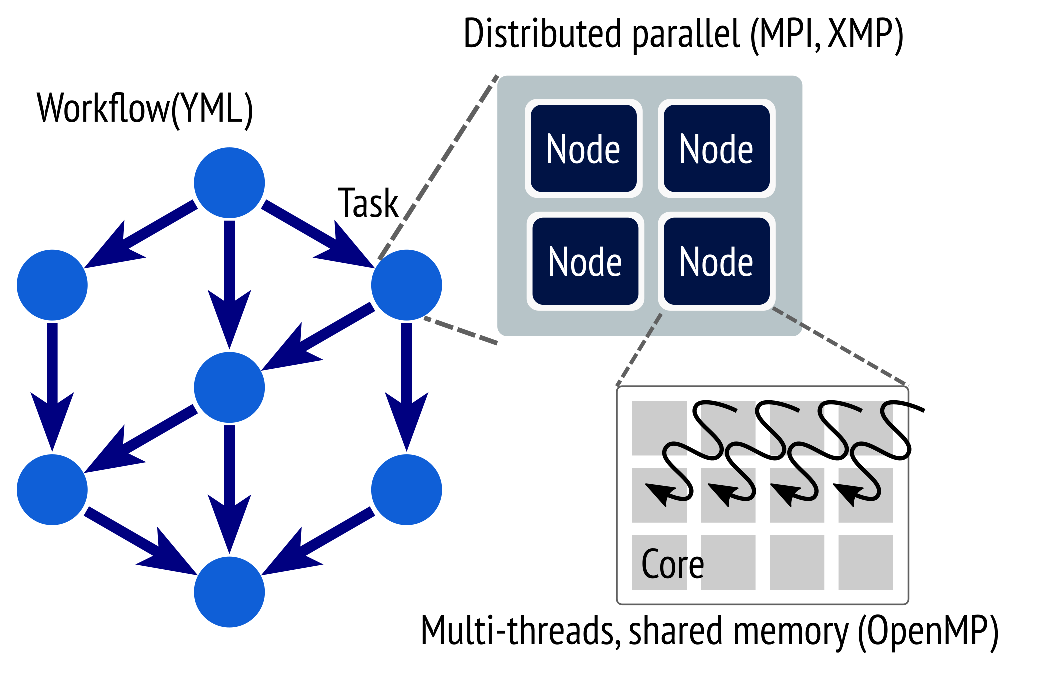
\includegraphics{img/mSPMD-overview.eps}}  
\caption{An overview of multi-SPMD programming model}
\label{figure:overview of mSPMD}
 \end{center}
\end{figure}

While most of programming model consider MPI+X such as MPI+OpenMP,  or MPI+X$_{1}$+X$_{2}\cdots $, we consider X$_{1}$+MPI (or XMP) +X$_{2}$ and propose a multi-SPMD (mSPMD) programming model where MPI programs and OpenMP+MPI programs work together in the context of a workflow programming model. In other words, tasks in a workflow are parallel programs written in XMP, MPI or their hybrid with OpenMP. 

Fig. \ref{figure:overview of mSPMD} shows the overview of the mSPMD programming model. 
In the target systems we has expected, there should be non-uniform memory access (NUMA) general purpose many cores and accelerators such as GPU. 
We  employ shared memory programming model in a node, or in a group of cores, and GPGPU programming in an accelerator. In a group of nodes, we have consider a distributed parallel programming model. Between these groups of nodes, there is a workflow programming model to manage and control several distributed parallel programs and hybrid programs of the distributed parallel and shared programming models.
To realize this framework, we support XcalableMP (XMP) to describe the distributed parallel programs in a workflow as well as MPI, which is a de-facto standard for distributed parallel programming.
For the shared programming and GPGPU, as well as XMP+OpenMP, MPI+OpenMP, MPI+GPGPU such as cuda, OpenACC, we support a runtime library called StarPU. The StarPU library\cite{Augonnet2011starpu}, which is a task programming library for hybrid architectures, enables us to implement heterogeneous applications in a uniform way. 
XMP provides an extension to enable work sharing among CPU cores and GPU \cite{odajima2013Adaptive}.
YML\cite{delannoy2004a, delannoy2006a, delannoy2006b}, a development and execution environment for a scientific workflow, is used to for the workflow execution. 

\subsection{YML}

\begin{figure}[t]
 \begin{center}
  \scalebox{0.22}{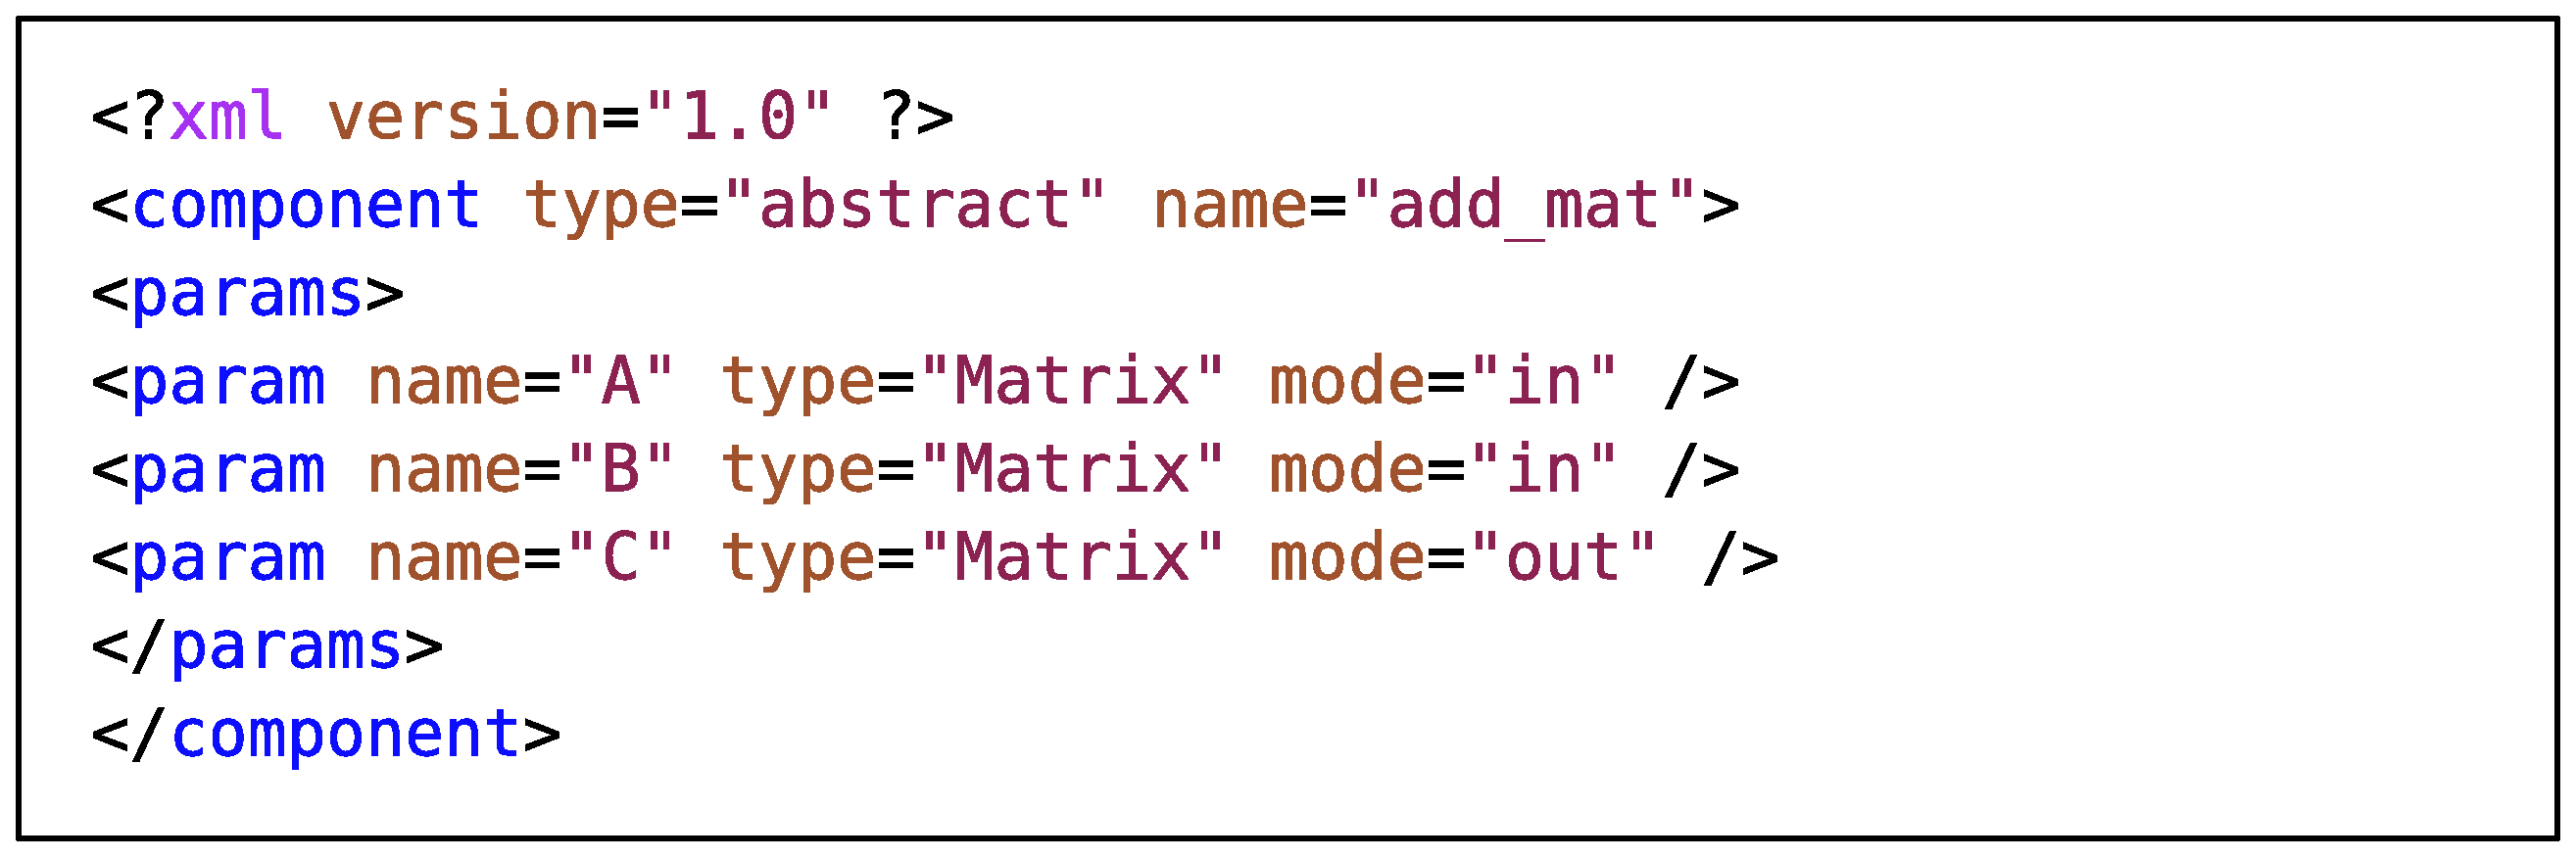
\includegraphics{img/abstract.eps}}
  \caption{An example of ``Abstract'' in YML}
  \label{fig:abstract component}
~\\
  \scalebox{0.22}{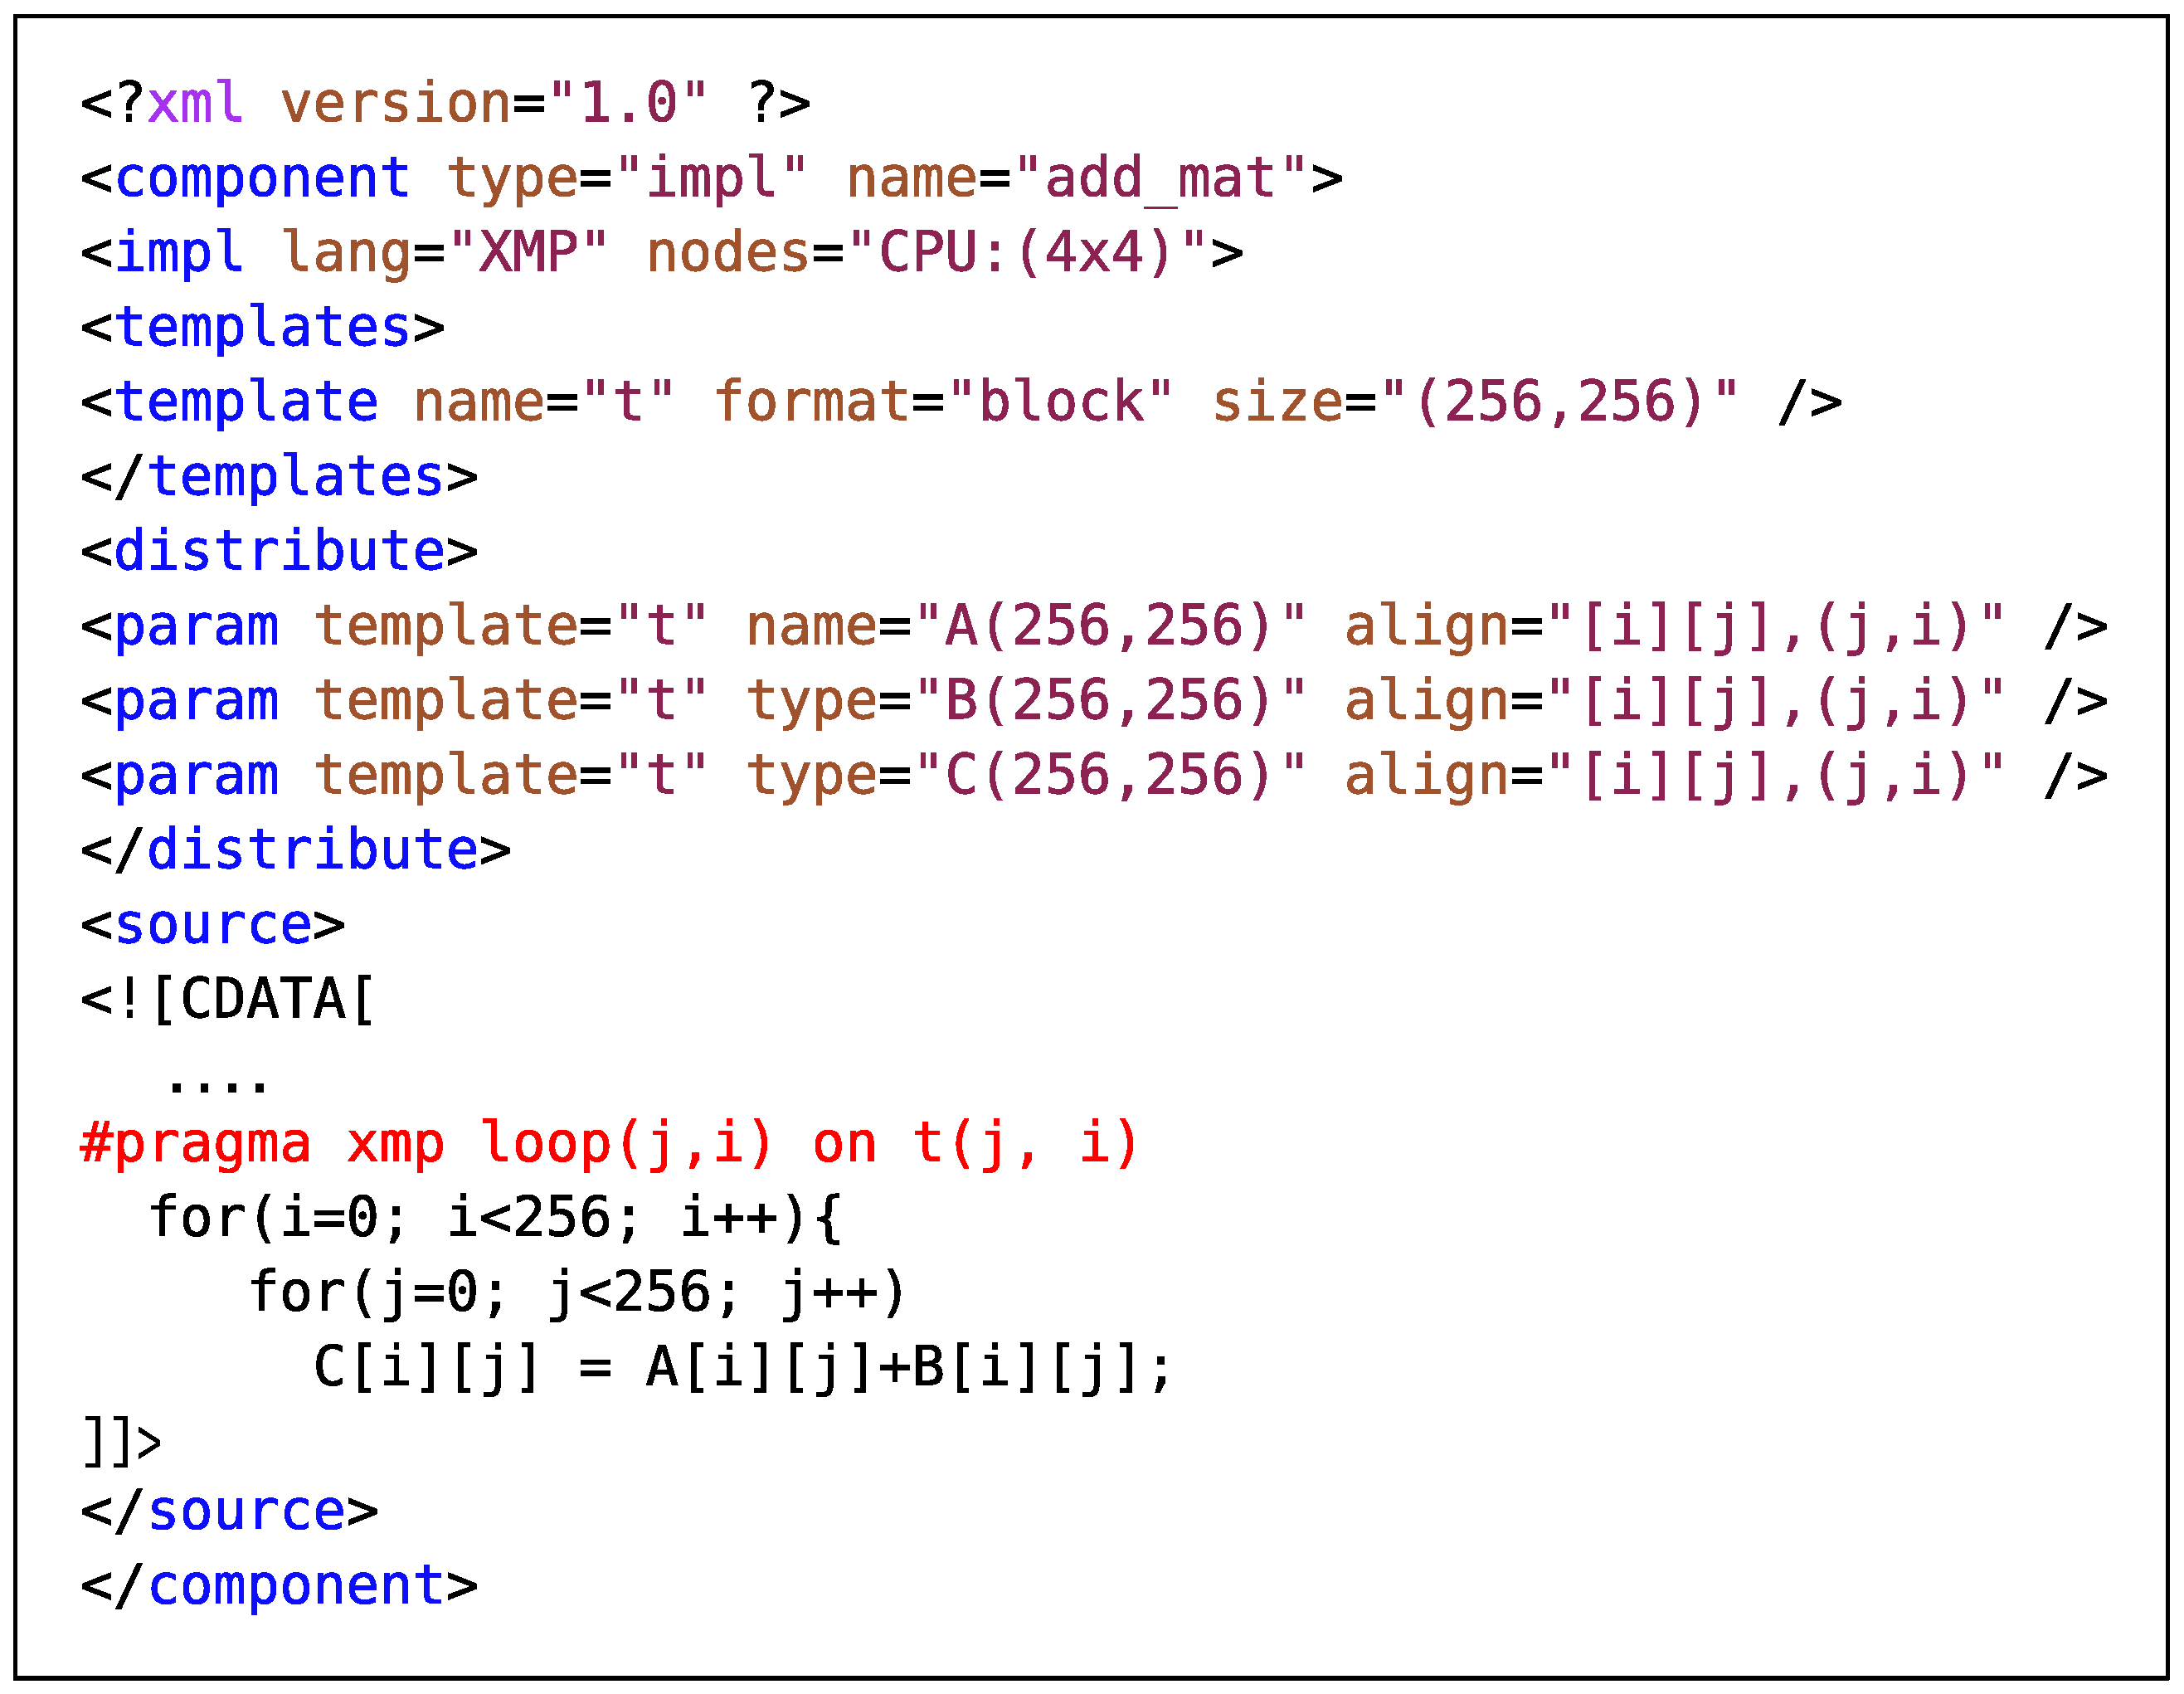
\includegraphics{img/impl.eps}}
  \caption{An example of ``Implementation'' in YML}
  \label{fig:impl component}
 \end{center}
\end{figure}

YML\cite{delannoy2004a, delannoy2006a, delannoy2006b} is a workflow programming environment for a scientific workflow. YML had been developed to execute a workflow application in grid and P2P environment and provides the following software:
\begin{itemize}
 \item Component (task) generator,  
 \item Workflow compiler and 
 \item Workflow scheduler.
\end{itemize}
The YML workflow compiler supports an original workflow language called YvetteML, which allow us to describe dependency between tasks easily. 
Some details of the YvetteML are described later, in section. \ref{subsection:workflow-yvettml}.
A workflow written in the YvetteML would be compiled by the YML workflow compiler into a DAG of tasks. The YML workflow scheduler interprets the DAG to execute the defined workflow. Depending on the available systems, the scheduler uses different middleware, such as XtremWeb for a P2P, OmniRPC\cite{sato2001a} for a grid. 
The YML component generator generate executable programs from ``abstract'' and ``implementation'' descriptions of a component. 
Figure \ref{fig:abstract component} and \ref{fig:impl component} show examples of ``abstract'' and ``implementation'' respectively. Note that in the figure \ref{fig:impl component}, while we show an example using XMP, the original YML had not supported neither XMP nor MPI. The XMP and MPI has supported by extending YML and middleware. 

\subsection{OmniRPC-MPI}
\label{subsection:omnirpc-mpi}

YML has been designed to execute workflow applications over various environments such as cluster, P2P and single processor.
During the execution, YML workflow scheduler dynamically load a backend library for its environment. 
Each of backend libraries calls APIs defined in middleware libraries. 
For example, in a grid environment, the OmniRPC backend linked with OmniRPC middleware library should be loaded. 

The OmniRPC \cite{sato2001a} is a grid RPC facility for cluster systems. The OmniRPC supports a master-worker programming model, where serial remote programs (rexs) are executed by exec, rsh or ssh. 

To realize mSPMD programming model, we have implemented MPI backend and extended the OmniRPC to OmniRPC-MPI for a large scale cluster environment.  
The OmniRPC-MPI library provides following functions:
\begin{itemize}
 \item invoke a remote program (worker program) over specified number of nodes
 \item communication between the workflow scheduler and the remote programs
       \begin{itemize}
	\item the scheduler sends a request to execute a certain task to a remote program
	\item the scheduler listens to communicator and receives a termination message from a remote program
       \end{itemize}
 \item manage remote programs and computational resources
\end{itemize}

\section{Application Development in the mSPMD programming environment}

In this chapter, we describe how to develop applications in the mSPMD programming environment. 

\subsection{Task generator}

\begin{figure}[t]
 \begin{center}
  \scalebox{0.25}{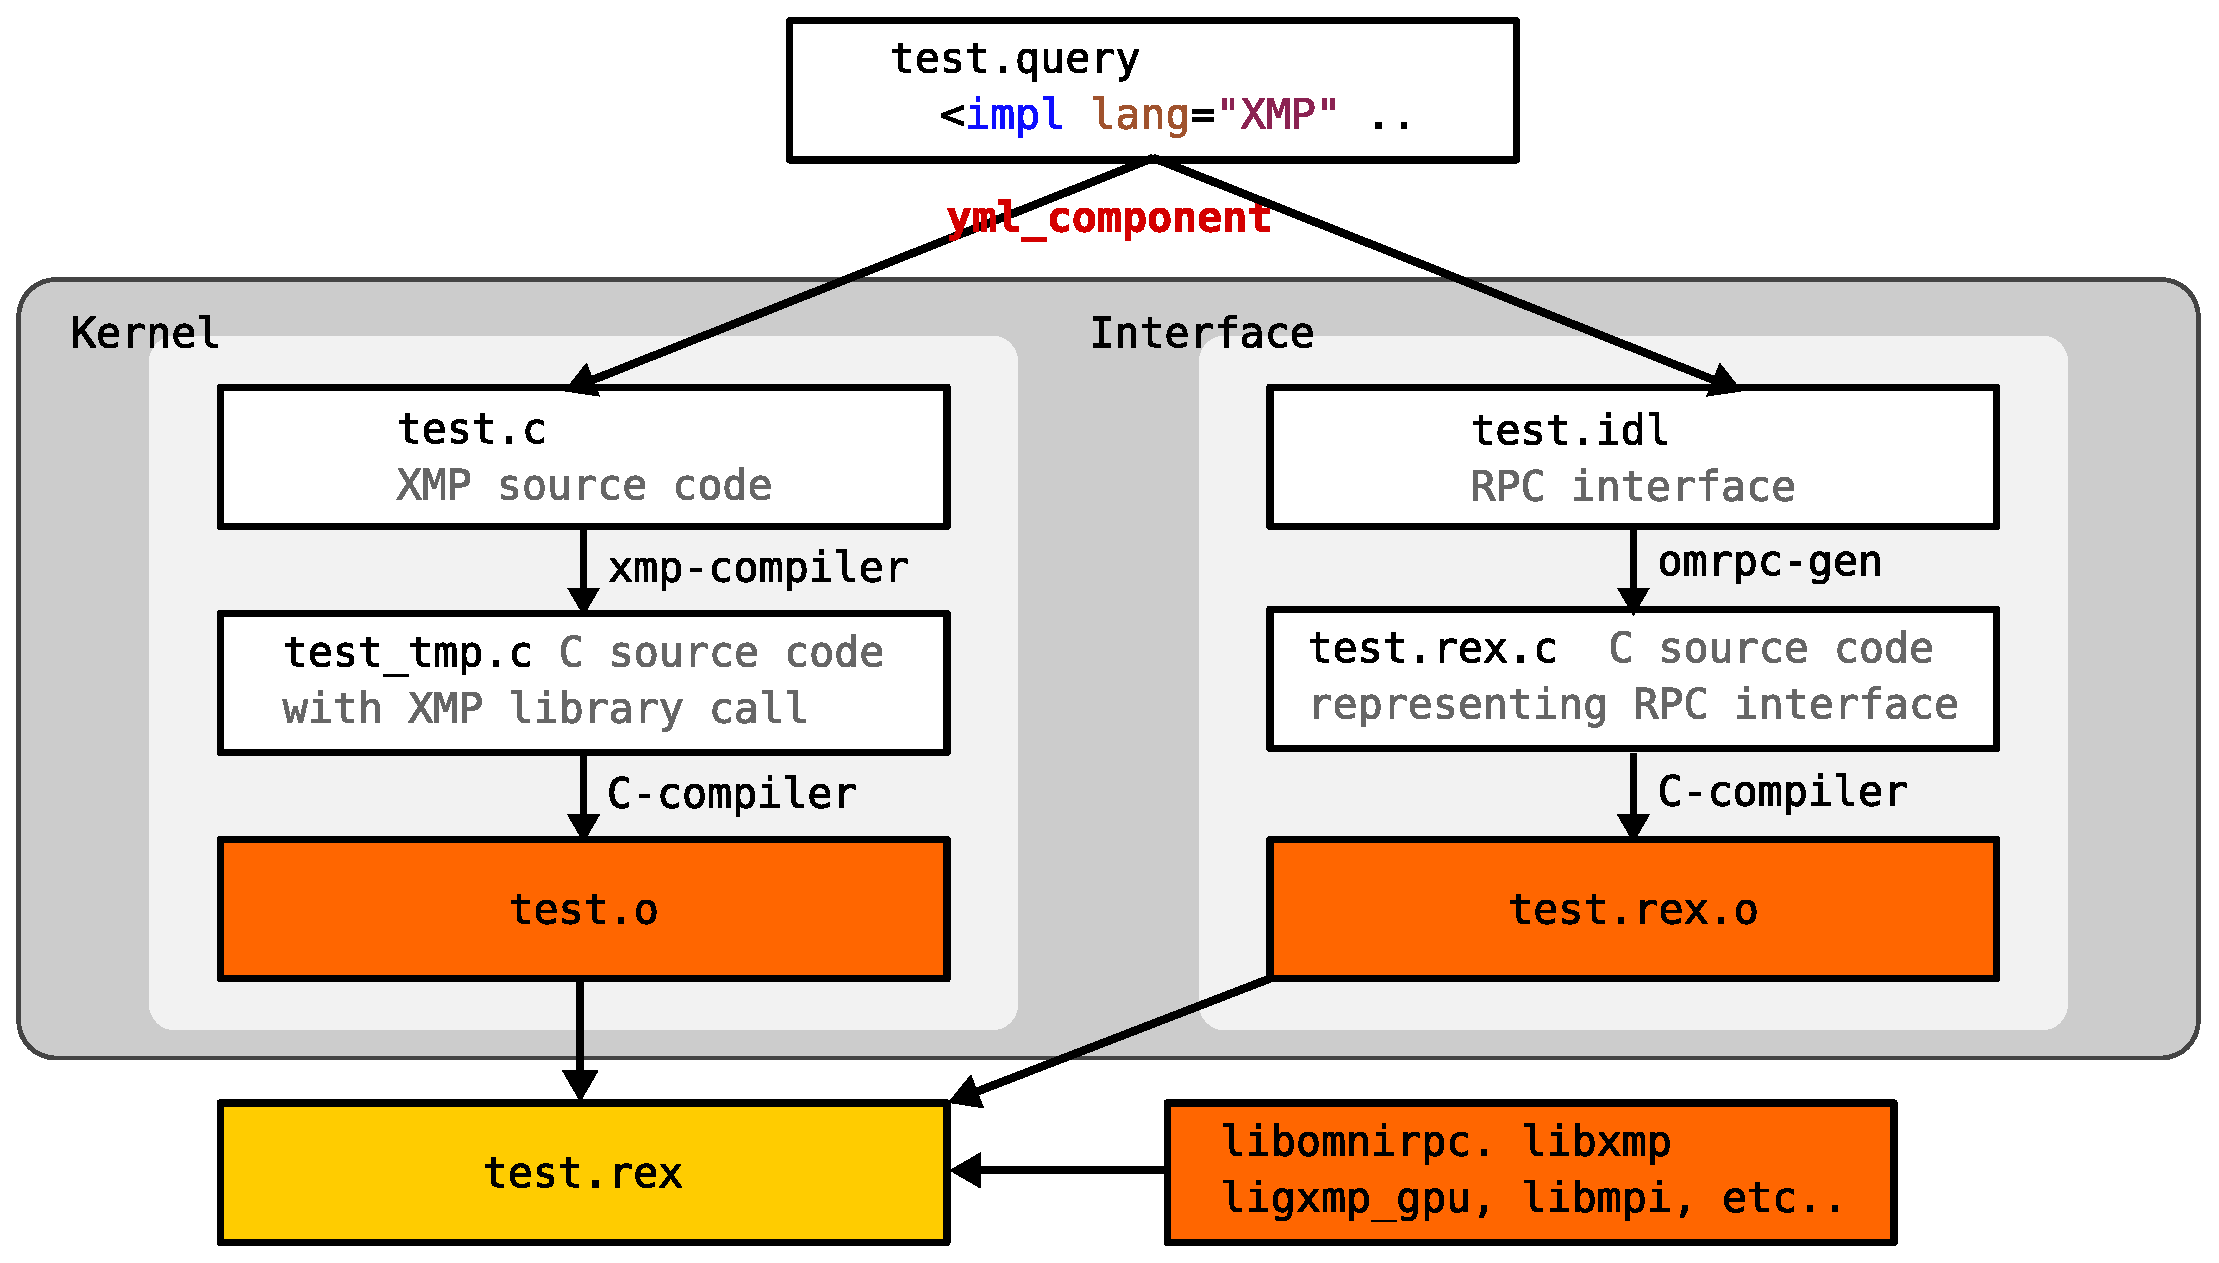
\includegraphics{img/task-generator.eps}}
  \caption{YML Component (task) generator extended for the mSPMD programming environment}
  \label{figure:task-generator}
 \end{center}
\end{figure}

Fig. \ref{figure:task-generator} shows the YML Component generator extended for the mSPMD programming environment. The generator takes an implementation source code such as the one shown in Fig. \ref{fig:impl component}. Then, combining the implementation and abstract source codes, it generate several intermediate files such as an XMP source code, which extracts task procedure itself defined by a user, and an interface definition file, which includes some communication functions used to communicate with a workflow scheduler. 
The YML Component generator calls (1) an xmp compiler to translate the XMP source code to a C-source code with XMP runtime library calls, and (2) a C-compiler to compile the C-source code generated by the XMP compiler. 
The YML Component generator calls (1) OmniRPC-generator to translate the interface definition to a C-source code, and (2) a C-compiler to compile the C-source code generated by the OmniRPC generator. Then, the YML Component generator calls a linker to link the compiled object files and external libraries such as an MPI library. 

During a workflow appliction execution, the remote programs generated by the YML Component generator are invoked and managed by the YML workflow scheduler and the OmniRPC-MPI middleware. 

\subsection{Workflow development}
\label{subsection:workflow-yvettml}

\begin{figure}[t]
 \begin{center}
  \scalebox{0.20}{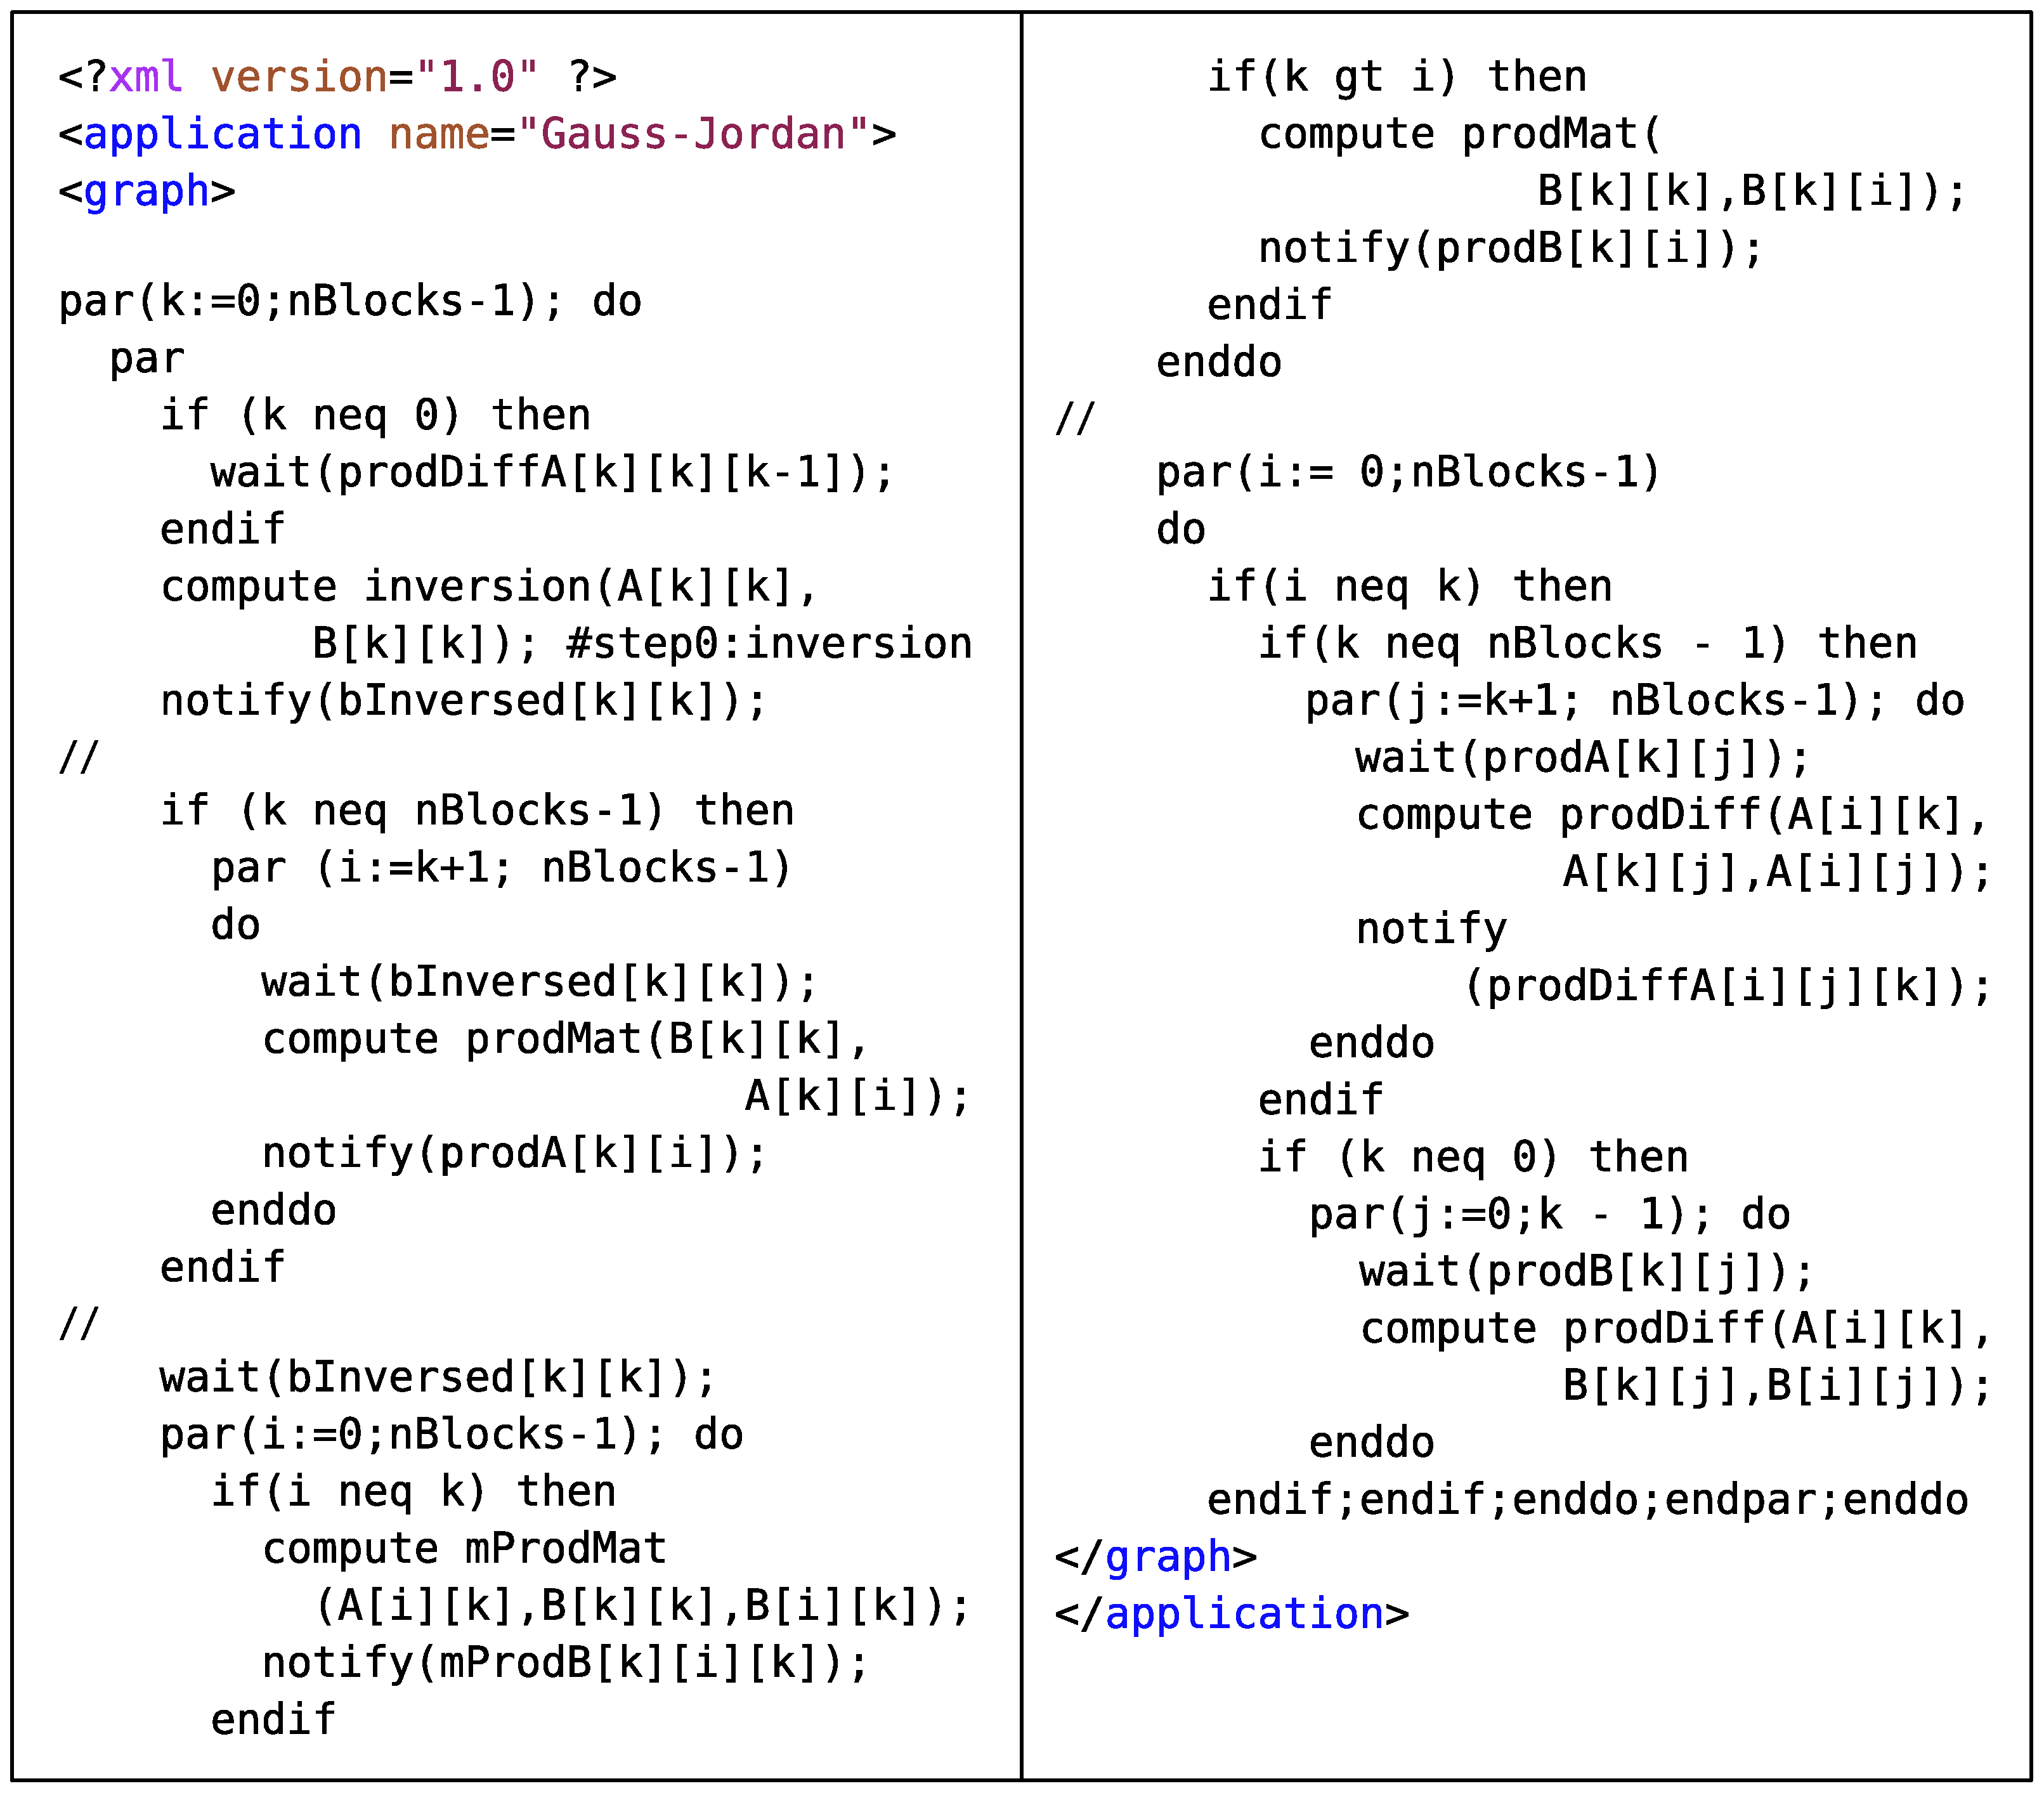
\includegraphics{img/application.eps}}
  \caption{An example of an application written in YvetteML}
  \label{figure:app-yvetteml}
 \end{center}
\end{figure}

A workflow application in the mSPMD is defined by a workflow description language called YvetteML. 
The YvetteML allows us to define the dependencies between tasks easily. 
Fig. \ref{figure:app-yvetteml} shows an example of the YvetteML, which computes an inversion of a matrix  by the block-Gauss-Jordan method. 
In the YvetteML, the following directives are supported:\\
\begin{tabular}[t]{rl}
 {\bf compute}& call a task \\
 {\bf par} & parallel loop or region\\
           & each index of the loop can be executed in parallel, or\\ 
           & each code block defined by {\bf // }in a {\bf par} region can be executed in parallel\\
 {\bf ser} & serial loop\\
 {\bf wait} & wait until the corresponding signal has been issued by {\bf notify}\\
 {\bf notify} & issues a specific signal for {\bf wait}
\end{tabular}

\subsection{Workflow execution}

\begin{figure}[t]
 \begin{center}
  \scalebox{0.20}{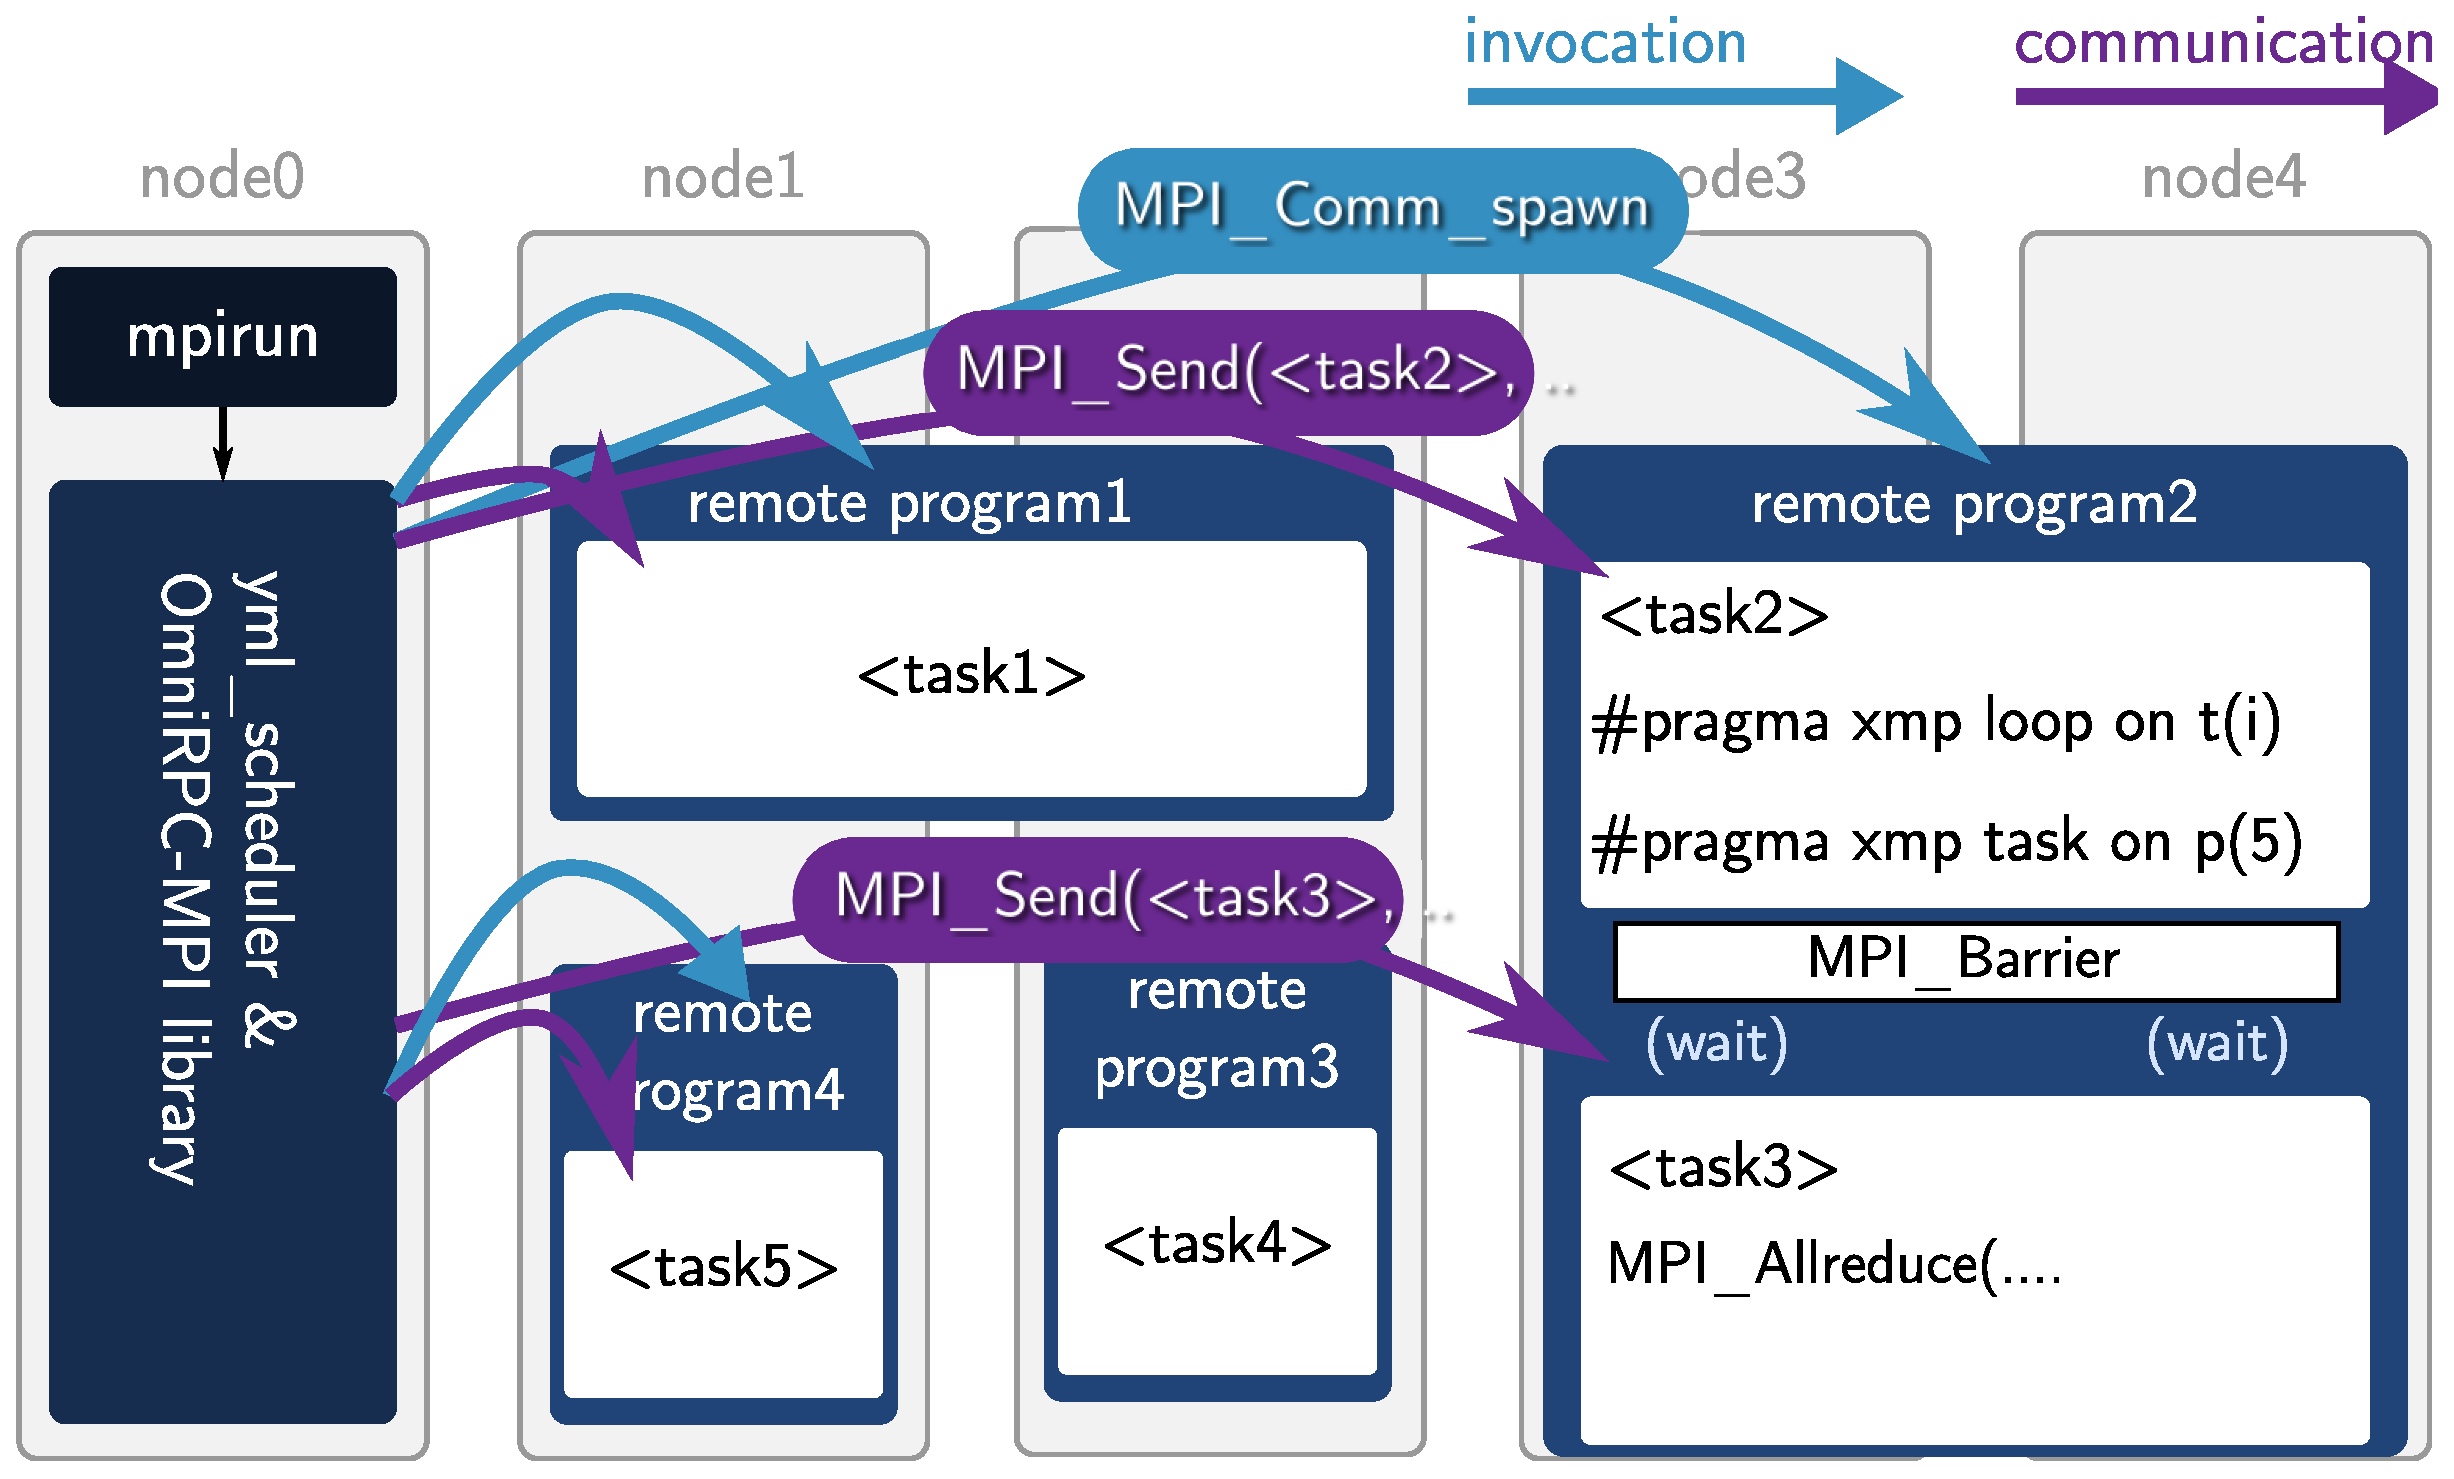
\includegraphics{img/workflow.eps}}
  \caption{A workflow execution of the mSPMD}
  \label{figure:app-execution}
 \end{center}
\end{figure}

The YML workflow compiler compiles the YvetteML into a directed acyclic graph (DAG), and the YML workflow scheduler interprets the DAG to execute a workflow application. 

Fig. \ref{figure:app-execution} illustrates a workflow execution in the mSPMD programming model. 
First, mpirun kicks the YML workflow scheduler. The YML workflow scheduler, which has been linked with the OmniRPC-MPI library, interprets the DAG of a workflow application and asks the invocation a task specified by YvetteML {\bf compute (task-name)} to the OmniRPC-MPI library. The OmniRPC-MPI library finds a remote program which includes the specified task, and invokes the remote program over the specified number of nodes by calling MPI\_Comm\_spawn, and sends a request to perform the specific task. 

While actual communications, node managements, and task scheduling have been supported by the OmniRPC-MPI library, the YML workflow scheduler schedules a ``logical'' order of tasks based on the DAG of an application.

\section{Experiments} 
\label{section:experiment}

\begin{table}[t]
\begin{center}
 \caption{Specification of K computer}
 \label{table:k-spec}
\begin{tabular}[t]{rrl}\hline\hline
 CPU & &Fujitsu SPARC64VIIIfx, 8 core, 2.00 GHz\\
Memory && 16GB , 64GB/s \\
Cache  && L1:32+32KB/core,  L2:6MB/core \\
Network & & Tofu (6D mesh/torus) Interconnect \\
        & & 5GB/s x 2 \\\hline
\end{tabular}
\end{center}
\end{table}

\begin{table}[t]
\begin{center}
\caption{Tasks in the Block Gauss Jordan workflow application. The input/output of the tasks such as $A_{i,j}, B_{i,j}, C_{i,j}, \cdots $ are blocks of a matrix }
\label{table:tasks}
\begin{tabular}[t]{rrl}\hline\hline
task&  & description \\\hline
inversion($A_{i,j}$) & ~~&compute the inversion of a block $A_{i,j}$ \\
prodMat($A_{i,j}$, $B_{i,j}$)& & compute $B_{i,j} =A_{i,j} B_{i,j}$ \\
mProdMat($A_{i,j}$, $B_{i,j}$,$C_{i,j}$) & &compute $C_{i,j} = - A_{i,j} B_{i,j}$\\
prodDiff($A_{i,j}$, $B_{i,j}$,$C_{i,j}$)  & &compute $C_{i,j} = C_{i,j}- A_{i,j} B_{i,j}$\\\hline
\end{tabular}

\end{center}\end{table}

In this section, we demonstrate the performance of the mSPMD programming model and our implementation. 

Table \ref{table:k-spec} shows the specification of the K-computer, which has been used for the experiments.


\begin{figure}[t]
\begin{center}
\begin{tabular}[t]{|ccc|}\hline
\hspace*{3mm}&
\begin{minipage}[c]{0.5\hsize}
~\\
{\bf for} $k$ {\bf from} $0$ {\bf to} $p-1$ {\bf do}\\
\hspace*{1.2em}(1) $Inv^{(k)} = [A_{k,k}^{(k)}]^{-1}$\\
\hspace*{1.2em}(2) $\bm{b}_k^{(k+1)}=Inv^{(k)}\cdot \bm{b}_k^{k}$\\
\hspace*{1.2em}{\bf if} $k \neq p-1$ {\bf then}\\
\hspace*{1.2em}\hspace*{1.2em}{\bf for} $i$ {\bf from} $0$ {\bf to} $p-1$ {\bf do}\\
\hspace*{1.2em}\hspace*{1.2em}\hspace*{1.2em}{\bf if} $i \neq k$ {\bf then}\\
\hspace*{1.2em}\hspace*{1.2em}\hspace*{1.2em}\hspace*{1.2em}(3) $A_{k,i}^{(k+1)}=Inv^{(k)}\cdot A_{k,i}^{(k)}$\\
\hspace*{1.2em}\hspace*{1.2em}\hspace*{1.2em}\hspace*{1.2em}(4) $\bm{b}_i^{(k+1)}=b_i^{(k+1)}-A_{i,k}^{(k)}\cdot \bm{b}_k^{(k+1)}$\\
\hspace*{1.2em}\hspace*{1.2em}\hspace*{1.2em}\hspace*{1.2em}{\bf for} $j$ {\bf from} $k+1$ {\bf to} $p-1$ {\bf do}\\
\hspace*{1.2em}\hspace*{1.2em}\hspace*{1.2em}\hspace*{1.2em}\hspace*{1.2em}(5) $A_{i,j}^{(k+1)} = A_{i,j}^{(k)}-A_{i,k}^{(k+1)}\cdot A_{k,j}^{(k)}$\\
\hspace*{1.2em}\hspace*{1.2em}\hspace*{1.2em}\hspace*{1.2em}{\bf end for}\\
\hspace*{1.2em}\hspace*{1.2em}\hspace*{1.2em}{\bf end if}\\
\hspace*{1.2em}\hspace*{1.2em}{\bf end for}\\
\hspace*{1.2em}{\bf end if}\\
{\bf end for}\\
\end{minipage}
&\hspace*{3mm}
\\\hline
\end{tabular}
\caption{Algorithm of the Block Gauss Jordan method}
\label{fig:block-gauss-jordan-algorithm}
\end{center}
\end{figure}

\begin{table}[t]
\begin{center}
\caption{\# of blocks, Block sizes and \# of tasks in the Block Gauss Jordan method}
\label{table:num blocks}
 \begin{tabular}[t]{r|r|r|r|r|r}\hline\hline
\# of blocks  & 1x1 & 2x2 & 4x4& 8x8& 16x16\\\hline
block size    & 32768$^2$ & 16384$^2$ & 8192$^2$ & 4096$^2$ & 2048$^2$ \\\hline
\# of tasks   & 3 & 18 & 108 & 696 & 4848 \\\hline
 \end{tabular}
\end{center}
\end{table}
 
In our experiments, Block Gauss-Jordan (BGJ) method, which computes the inversion of a matrix $A$, has been considered. 
Fig. \ref{fig:block-gauss-jordan-algorithm} shows the algorithm of the BGJ method. The workflow for the BGJ method written in YvetteML has been shown in Fig. \ref{figure:app-yvetteml}.
As shown in the table \ref{table:tasks}, 
tasks in the workflow process block(s). 
In order to investigate the performance over different levels of hierarchical parallelism:
\begin{itemize}
 \item the total size of the matrix $A$ is fixed to $32768\times 32768$, but the number of blocks is varied from $1\times1$ to $16 \times 16$. 
 \item the total number of processes (cores) for a workflow is fixed to $4096$, but the number of processes for each task is varied from 8 to 4096. 
\end{itemize}
Therefore, if we have a single block and assign all processes for a task, then it is almost equivalent to a distributed parallel application. 
On the other hand, if we divide a matrix into many small blocks and assign a process for each block, it is almost a traditional workflow application. 
Table \ref{table:num blocks} shows the block size and the number of tasks for each the number of blocks.
If we assign 512 processes for each task, then at most 8 tasks can be executed simultaneously. 


\begin{figure}[t]
 \begin{center}
  \scalebox{0.8}{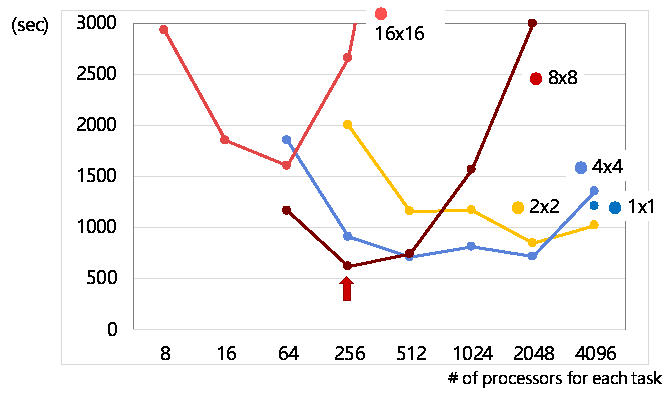
\includegraphics{img/result.eps}}
 \end{center}
 \caption{Execution time of the BGJ workflow applications}
\label{fig:result-bgj}
\end{figure}

Figure \ref{fig:result-bgj} shows the execution time of the BGJ workflow applications for the number of blocks and the number of  processes per task. 
The results show that the best performance has been realized when we divide a matrix into $8 \times 8$ blocks and assign 256 processes for each task. 
Our framework of the mSPMD programming model can realize such appropriate combination of different parallelisms and can allow application developers to control the different parallelism levels easily. 
On the other hand, the extreme cases --- $1 \times 1$ block and $16 \times 16$ blocks ---, have not performed well. Also, assigning too many processes for small tasks, for example 2048 processes for $8 \times 8$ blocks, more than 256 processes for $16 \times 16$ processes, show poor performance. 


\begin{figure}[t]
 \begin{center}
  \scalebox{0.3}{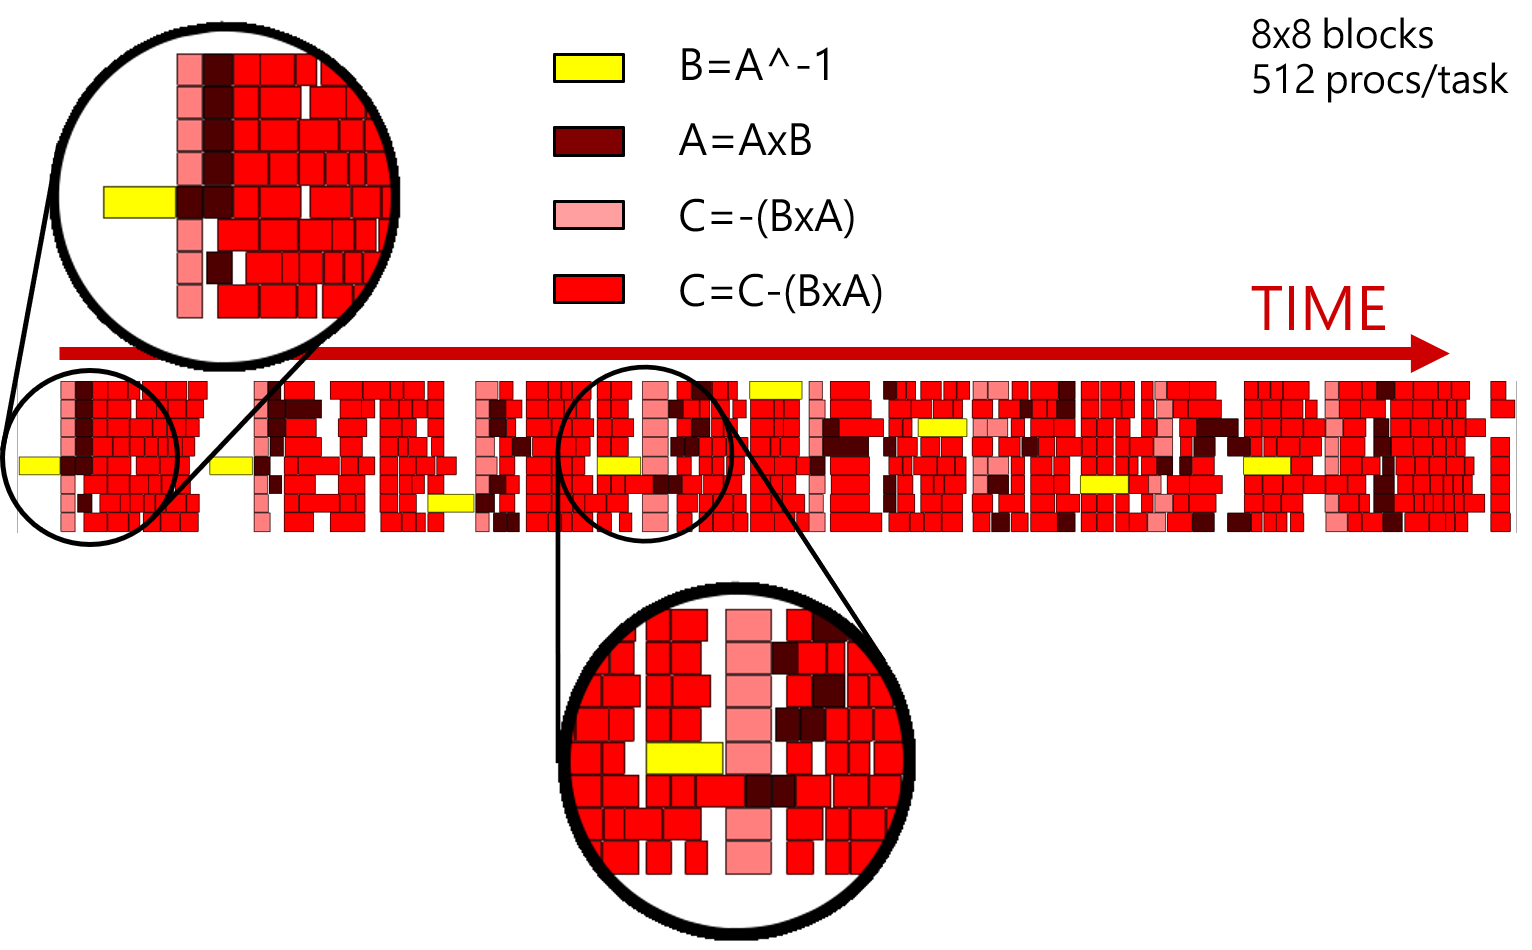
\includegraphics[bb=0 0 735 456]{img/timeline.png}}
 \end{center}
 \caption{Execution timeline of the BGJ workflow application with $8\times 8$ blocks}
\label{fig:timeline}\
\end{figure}

Figure \ref{fig:timeline} shows the execution timeline (from left to right) of the BGJ workflow application with $8\times 8$ blocks. As shown in the figure, at the first step, the task of inversion ($B=A^{-1}$) must be executed solely since the other tasks on the first step uses the result of the inversion. After the 2nd step, some of the matrix calculations such as $A=A\times B, C=-(B\times A), C=C-(B\times A)$ on the $k$-th step and the inversion on $k+1$-th step can be overlapped. For other programming models such as flat-MPI, it is not easy to execute tasks or functions on different steps simultaneously. On the other hand, the mSPMD programming model and our programming environment allow application developers to describe this sort of applications easily. 

\section{Eigen solver on the mSPMD programming model}

In this section, as a use case of the mSPMD programming model, 
we introduce an eigen solver implemented on the mSPMD programming model. 

\subsection{Implicitly Restarted Arnoldi Method (IRAM), Multiple Implicitly Restarted Arnoldi Method (MIRAM) and their implementations for the mSPMD programming model} 

The iterative methods are widely used to solve eigen programs in scientific computation. 
Implicitly Restarted Arnoldi Method (IRAM) \cite{Sorensen-iram} is one of the iterative methods to search the eigen elements $\lambda$ s.t. $A \bm{x} = \lambda \bm{x} $ of a matrix $A$. 

\begin{figure}[t]
\begin{tabular}[t]{|ccc|}\hline
\hspace*{3mm}&
\begin{minipage}[c]{0.9\hsize}
~\\
Input: $A, V_m, H_m, F_m$ with $A V_m = V_m H_m+f_m e_m$\\
\hspace*{1.2em}$A$ is a matrix of order $n$, \\
\hspace*{1.2em}$m$ is krylov subspace size s.t. $m\ll n$,\\
\hspace*{1.2em}$k$ is the number of desired eigen pairs s.t. $k<m$.\\
{\bf for} $i$ {\bf from} $0$ {\bf to} convergence {\bf do}\\
\hspace*{1.2em}(1) compute the eigenvalue $\sigma$ and eigenvectors of $H_m$\\
\hspace*{1.2em}compute residual norm. If converge, stop.\\
\hspace*{1.2em}(2) Select a set of $p=m-k$ shifts $(u_1,\cdots,u_p)$ and set $q^T:=e_m^T$\\
\hspace*{1.2em}(3) {\bf for} $j$ {\bf from } $1$ {\bf to} $p$\\
\hspace*{1.2em}\hspace*{1.2em} (1)  $\mbox{Factor}[Q_j,R_j] = \mbox{qr}(H_m-u_jI)$\\
\hspace*{1.2em}\hspace*{1.2em} (2) $H_m = Q_j^T H_m Q_j$, $V_m=V_mQ_j$\\
\hspace*{1.2em}\hspace*{1.2em} (3) $q^H=q^H Q_j$\\
\hspace*{1.2em}{\bf end for}\\
\hspace*{1.2em}(4) $f_k = v_{k+1}\beta_k + f_m \sigma_k$, $V_k=V_m(1:n, 1:k)$, $H_k=H_m(1:k,1:k)$\\
\hspace*{1.2em}(5) Apply $p$ additional steps of Arnoldi process to obtain a new $m$ step Arnoldi \\
\hspace*{1.2em}factorization $AV_m = V_m H_m +f_m e_m^T$\\
{\bf end for}\\
\end{minipage}
&\hspace*{3mm}
\\\hline
\end{tabular}
\caption{Algorithm of IRAM}
\label{fig:iram-algorithm}
\end{figure}

Figure \ref{fig:iram-algorithm} shows the algorithm of IRAM. IRAM is 
 a technique that combines the implicitly shifted QR mechanism with an Arnoldi factorization and the IRAM can be viewed as a truncated form of the implicitly shifted QR-iteration.
After the first $m$-step Arnoldi factorization, the eigen pairs of Heisenberg matrix $H$ are computed. If the residual norm is enough small, the iteration is stopped. Otherwise, the shifted QR by selecting shifts based on eigenvalues of the Heisenberg matrix is computed. 
Using these new vectors and $H$ as a starting point, we can apply $p$ additional steps of the Arnoldi process to obtain an $m$-step Arnoldi factorization. 

Multiple IRAM (MIRAM) is an extension of IRAM, which introduce two or more instances of IRAM. 
The instances of IRAM work on the same problem, but they are initialized with different subspaces $m_1, m_2,\cdots $. 
At the restarting point, each instance selects the best $(m_{best}, H_{best}, V_{best}, f_{best})$ from $l$ IRAM instances. 

\begin{figure}[t]
\begin{tabular}[t]{cc}
\begin{minipage}[c]{0.5\hsize}
\begin{center}
 \scalebox{0.30}{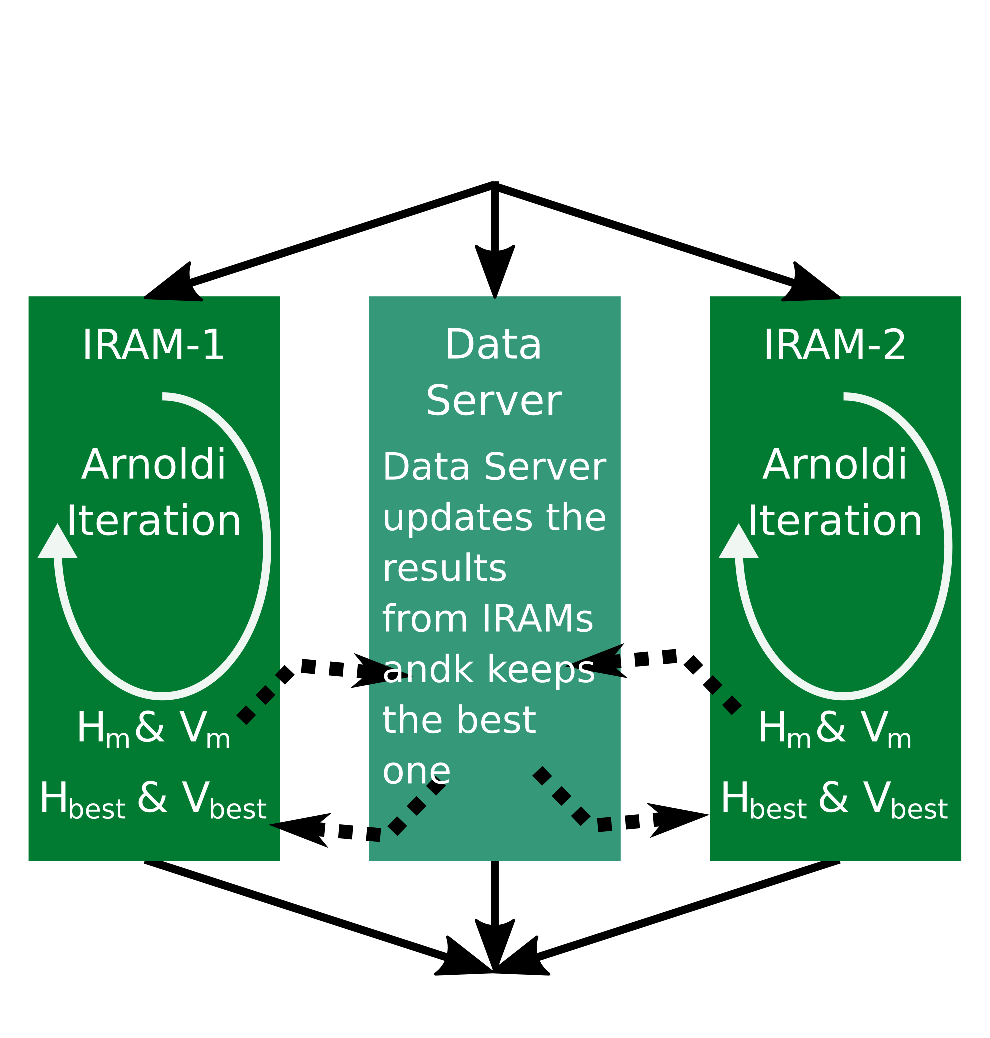
\includegraphics[angle=0]{img/miram-overview.eps}} 
 \caption{Overview of MIRAM on the mSPMD programming model}
 \label{fig:overview-miram}
\end{center}
\end{minipage}
 & 
\begin{minipage}[c]{0.4\hsize}
\begin{center}
 \scalebox{0.22}{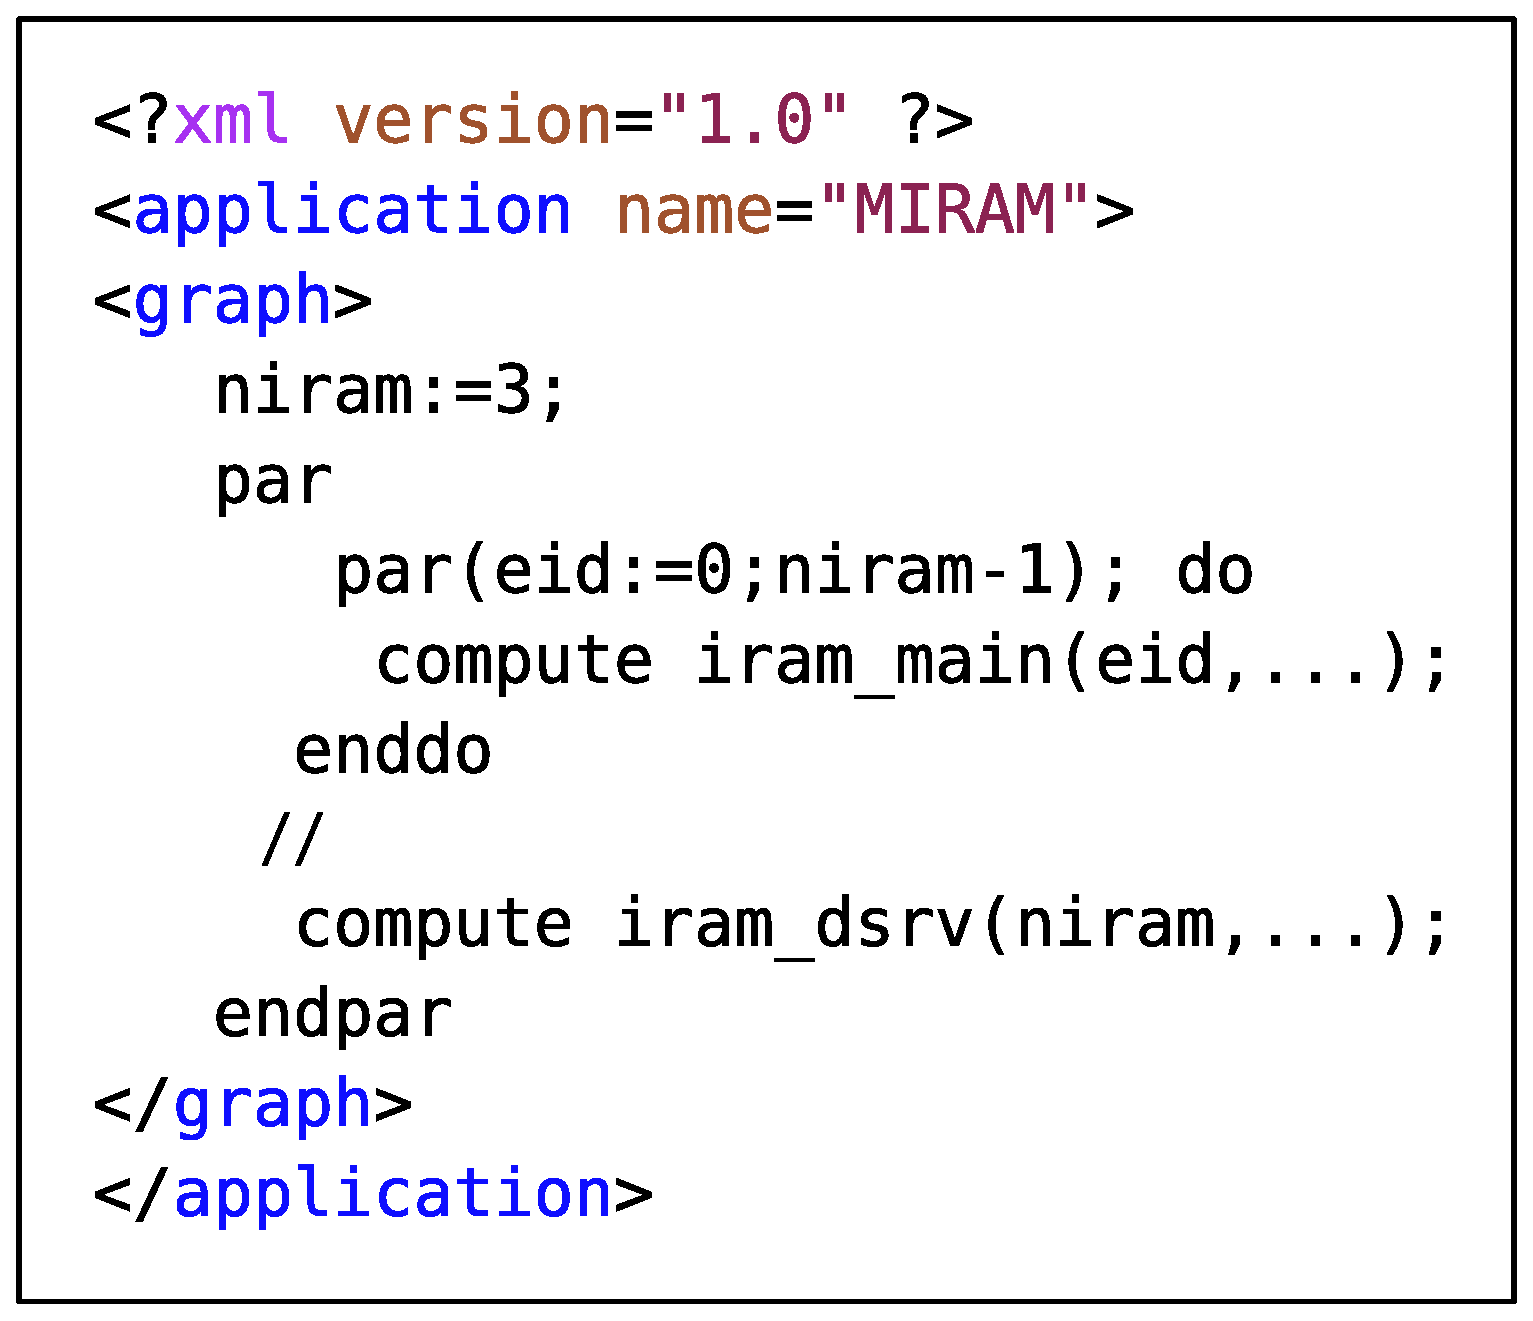
\includegraphics{img/miram-application.eps}} 
 \caption{MIRAM workflow}
 \label{fig:miram-workflow}
\end{center}
\end{minipage}
\\
\end{tabular}
\end{figure}

In the mSPMD programming model, MIRAM has been implemented as shown in Figure \ref{fig:overview-miram}. 
The source code written in YvetteML is shown in Figure \ref{fig:miram-workflow}. 
The YML workflow scheduler invokes $l$ IRAM instances and a data server. 
Each of IRAM instances computes Arnoldi iteration asynchronously over $n$ nodes, and sends 
resulted $(m, H, V, f)$ to the data server.  
The data server keeps the best result and send it to each IRAM. Each IRAM restarts with the $(m, H, V, f)$ sent by the data server. 

\subsection{Experiments}


\begin{table}[t]
\begin{center}
 \caption{Specification of T2K Tsukuba}
 \label{table:t2k-spec}
\begin{tabular}[t]{rrl}\hline\hline
 CPU & & Opteron Barcelona B8000, 4 cores, 4 sockets, 2.3 GHz\\
Memory && 32GB\\
Network & & Fat-tree, full-bisection interconnection quad-rail of InfiniBand\\\hline
\end{tabular}
\end{center}
\end{table}

Here, we show the result of experiments on T2K-Tsukuba supercomputer. The specification of the T2K Tsukuba is shown in Table \ref{table:t2k-spec}. 
In the experiments, we use a matrix called {\it Schenk/nlpkkt240} from the SuiteSparse Matrix Collection \cite{matrix-collection}, where $n=27,993,600$ and the number of non-zero elements are  760,648,352. 


\begin{figure}[t]
 \begin{center}
  \scalebox{1.0}{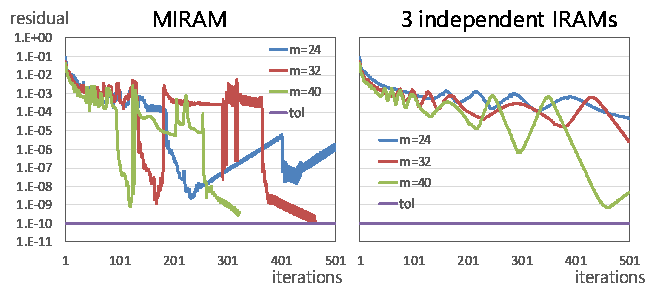
\includegraphics{img/miram-result.eps}}
  \caption{Results of MIRAM with 3 IRAM solvers (right) and 3 independent run of IRAM (left)}
  \label{figure:result-miram}
 \end{center}
\end{figure}

Figure \ref{figure:result-miram} shows the results of MIRAM with IRAM solvers of $m=24, 32, 40$ 
 (left) and 3 independent run of IRAM solvers of the $m=24, 32, 40$ (right). While MIRAM converged around 450 iterations, non of 3 IRAMs could not converge until 500 iterations. 

 This MIRAM example shows that by using the mSPMD programming model, two different accelerations can be achieved. While the workflow programming model of the mSPMD accelerates convergence of the Arnoldi iterations, the distributed parallel programming model speeds up each iteration of the Arnoldi method. 


\section{Fault Tolerance Features in the mSPMD programming model}
\label{section:fault tolerance}

\subsection{Overview and implementation}

As well as scalability and programmability, reliability is important issue in the exascale computing. Since the number of components of an exascale supercomputer should be tremendously large, it is obvious that the mean time between failure (MTBF) of a system decreases as the number of the system's components increases.  
Therefore, fault tolerance becomes important for systems and applications. 
Here, we develop a fault tolerance mechanism in a mSPMD programming model and it's development and execution environment. The fault tolerance in the mSPMD programming model can be realized without modifying applications' source codes\cite{tsuji2015i}. 


\begin{figure}[t]
 \begin{center}
  \scalebox{0.20}{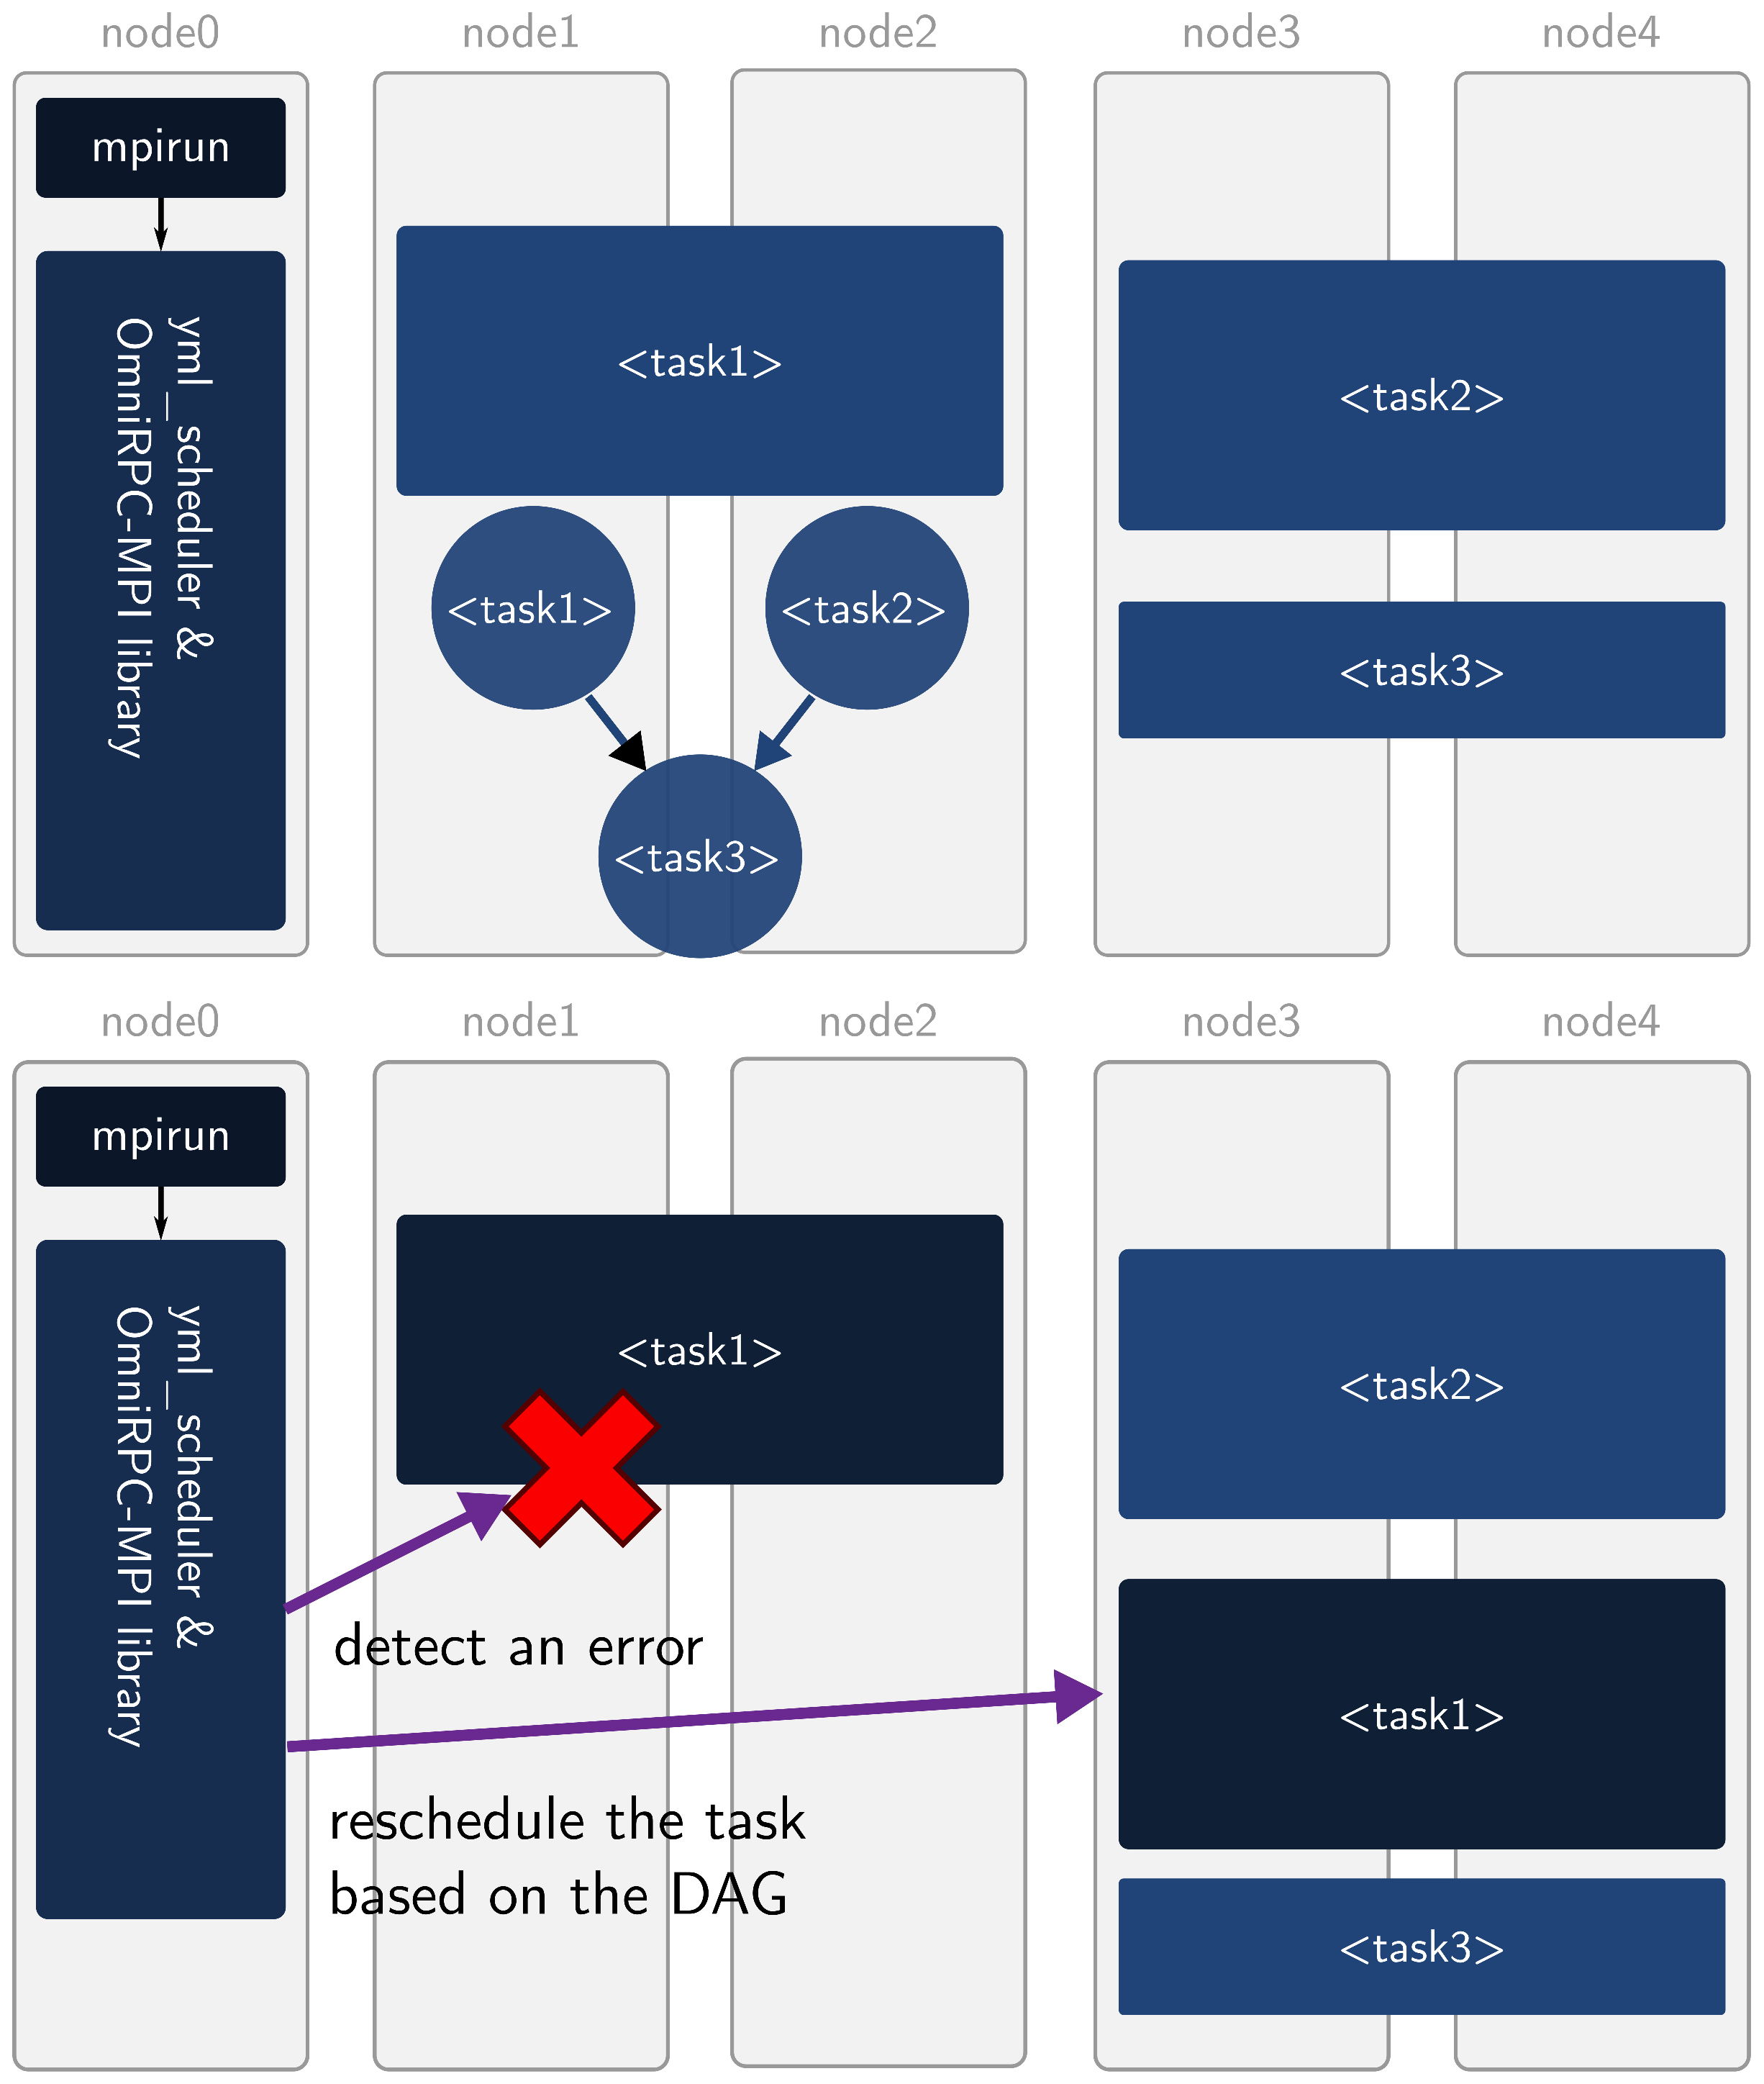
\includegraphics{img/workflow-ft.eps}}
\caption{Overview of fault tolerance in the mSPMD programming model}
\label{fig:overview-ft}
 \end{center}
\end{figure}

Figure \ref{fig:overview-ft} illustrates the fault tolerant mechanism in the mSPMD programming model. If the workflow scheduler can find an error in a task and execute the task again on different nodes, then we can realize a fault tolerance and resilience mechanism automatically. 

We have extended the OmniRPC-MPI described in \ref{subsection:omnirpc-mpi} to detect errors in remote programs and notify the errors to the YML workflow scheduler. For these purposes, heartbeat messages between master and remote programs has been introduced in the OmniRPC-MPI library. 
If an error is detected in a remote program, then it is reported to the YML workflow scheduler as a return value of existing APIs. 
The {\tt OmniRpcProbe(Request r)} API has been designed to listen the status of a requested task in a remote program. This returns {\tt success} if the remote program sends a signal to indicate the requested task {\tt r} has successfully finished. 
On the other hand, if heartbeat messages from the remote program executing the task {\tt r} have stopped, {\tt OmniRpcProbe(Request r)} returns {\tt fail}.

The YML scheduler re-scheduler the failed task if it receives {\tt fail} signal from the OmniRPC-MPI library. 
The re-scheduling method is simple; The YML scheduler puts the failed task at the head of the ``ready'' task-queue. 

\subsection{Experiments}

\begin{table}[t]
\begin{center}
 \caption{Specification of a FX10 cluster}
\label{table:fx10-spec}
\begin{tabular}[t]{rrl}\hline\hline
 CPU & &Fujitsu SPARC64VIIIIfx, 16 core, 1.65 GHz\\
Memory && 32GB, 85GB/s \\
Cache  && L1:32+32KB/core,  L2:6MB/core \\
Network & & Tofu (6D mesh/torus) Interconnect \\
        & & 5GB/s x 2 \\\hline
\end{tabular}
\end{center}
\end{table}


We have performed some experiments to investigate the overhead of the fault detection and the elapsed time when errors occur on a cluster shown in Table \ref{table:fx10-spec}.
The BGJ method shown in section \ref{section:experiment} had been used.
The size of a matrix is $20480\times 20480$ and divided into \\
\hspace*{20mm}
\begin{tabular}[t]{r|r|r|r|r}\hline\hline
\# of blocks  & 1x1 & 2x2 & 4x4& 8x8\\\hline
block size    & 20480$^2$ & 10240$^2$ & 5120$^2$ & 2560$^2$\\\hline
\end{tabular}\\
1024 cores (64 nodes) are used for each workflow, and 64 to 1024 cores are assigned for each task in a workflow. 


\begin{figure}[p]
 \begin{center}
  \begin{tabular}[t]{c}
   \begin{minipage}[t]{0.90\hsize}
\hspace*{10mm}    \scalebox{1.0}{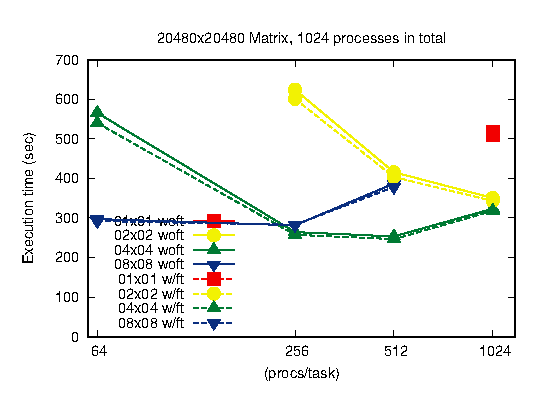
\includegraphics{img/etime_20480_1024_0000000-1.eps}}\\
    \vspace*{20mm}
    \caption{Execution time with and without FT for the number of cores for each task. The graph legends show the number of blocks.}
    \label{fig:exectime-hb-overhead}
   \end{minipage}
\\
   \begin{minipage}[t]{0.90\hsize}
    \hspace*{10mm}    \scalebox{1.0}{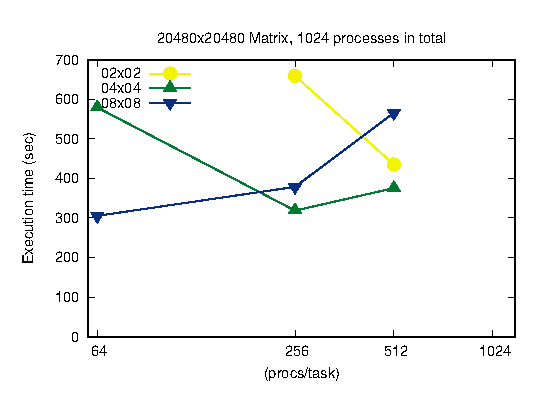
\includegraphics{img/etime2_20480_1024_0090000.eps}}   \\
    \vspace*{20mm}
    \caption{Execution time with FT for the number of cores for each task under fake errors. The graph legends show the number of blocks.}
    \label{fig:exec-time-w-errors}
   \end{minipage}
       \\
  \end{tabular}
 \end{center}
\end{figure}

Firstly, we have considered the overhead of the heartbeat messages used to detect errors in remote programs. 
Figure \ref{fig:exectime-hb-overhead} shows the performance of 
the normal and fault tolerant mSPMD programming executions using between 64 and 1024 compute cores per a task. 
The dotted lines are the results of fault tolerant mSPMD programming executions and the solid lines are those of the normal mSPMD programming executions. As shown in the figure, the best combination of the number of blocks and the number of processes per task is $4\times 4$ blocks and 512 processes for the both cases of with and without fault tolerance support. 
The overhead of using heartbeat message is very small, and is 2.3\% on average and 4.7\% at a maximum.

Then, we have investigated the behavior and performance of the fault tolerant mSPMD programming execution when errors occur. 
Instead of waiting real errors, we have inserted fake errors that stop heartbeat messages from remote programs randomly with a certain error probability computed by an expected MTBF (90,000 sec). 
Figure \ref{fig:exec-time-w-errors} shows the performance of the fault tolerant mSPMD programming execution under the fake errors. Unfortunately, for the case of $1\times 1$ block and 1024 processes per task, it was not possible to complete the workflow, since the face error ratio used in the experiment is higher than real systems. 
For the other cases, the applications can be completed. 
The best combination of the number of blocks and the number of processes per task is $4 \times 4$ blocks and 256 processes while it was 512 processes under the ``no-error'' condition. This is because the tasks executed on relatively small number of nodes are relatively easy to recover when they fail. 

\section{Runtime correctness check for the mSPMD programming model}
\label{section:Runtime correctness check for the mSPMD programming model}

\subsection{Overview and implementation}

The mSPMD programming model has been proposed to realize scalability for large scale systems. Additionally, as we discussed at section \ref{section:fault tolerance}, we support fault tolerant features in the mSPMD programming model. 
In this section, we discuss about another important issue in large scale systems, productivity. 

One of the reasons for the low productivity in distributed parallel programs is the difficulty of debugging. 
To help to debug parallel programs, several libraries and tools have been proposed. 
MUST (Marmot Umpire Scalable Tool) \cite{MUST-project,Hilbrich2012must,Hilbrich2013must} is a runtime tool that provides a scalable solution for efficient runtime MPI error checking. The MUST has supported not only MPI but also XcalableMP (XMP) \cite{Protze2017a}. 

In this section, we discuss how to adopt the MUST library to the SPMD programs in the mSPMD programming model and enable the MUST correctness checking for the mSPMD.
Computational experiments have been performed to confirm MUST's operation in the mSPMD and to estimate the overhead of the correctness checking.

\begin{figure}[t]
 \begin{center}
\scalebox{0.20}{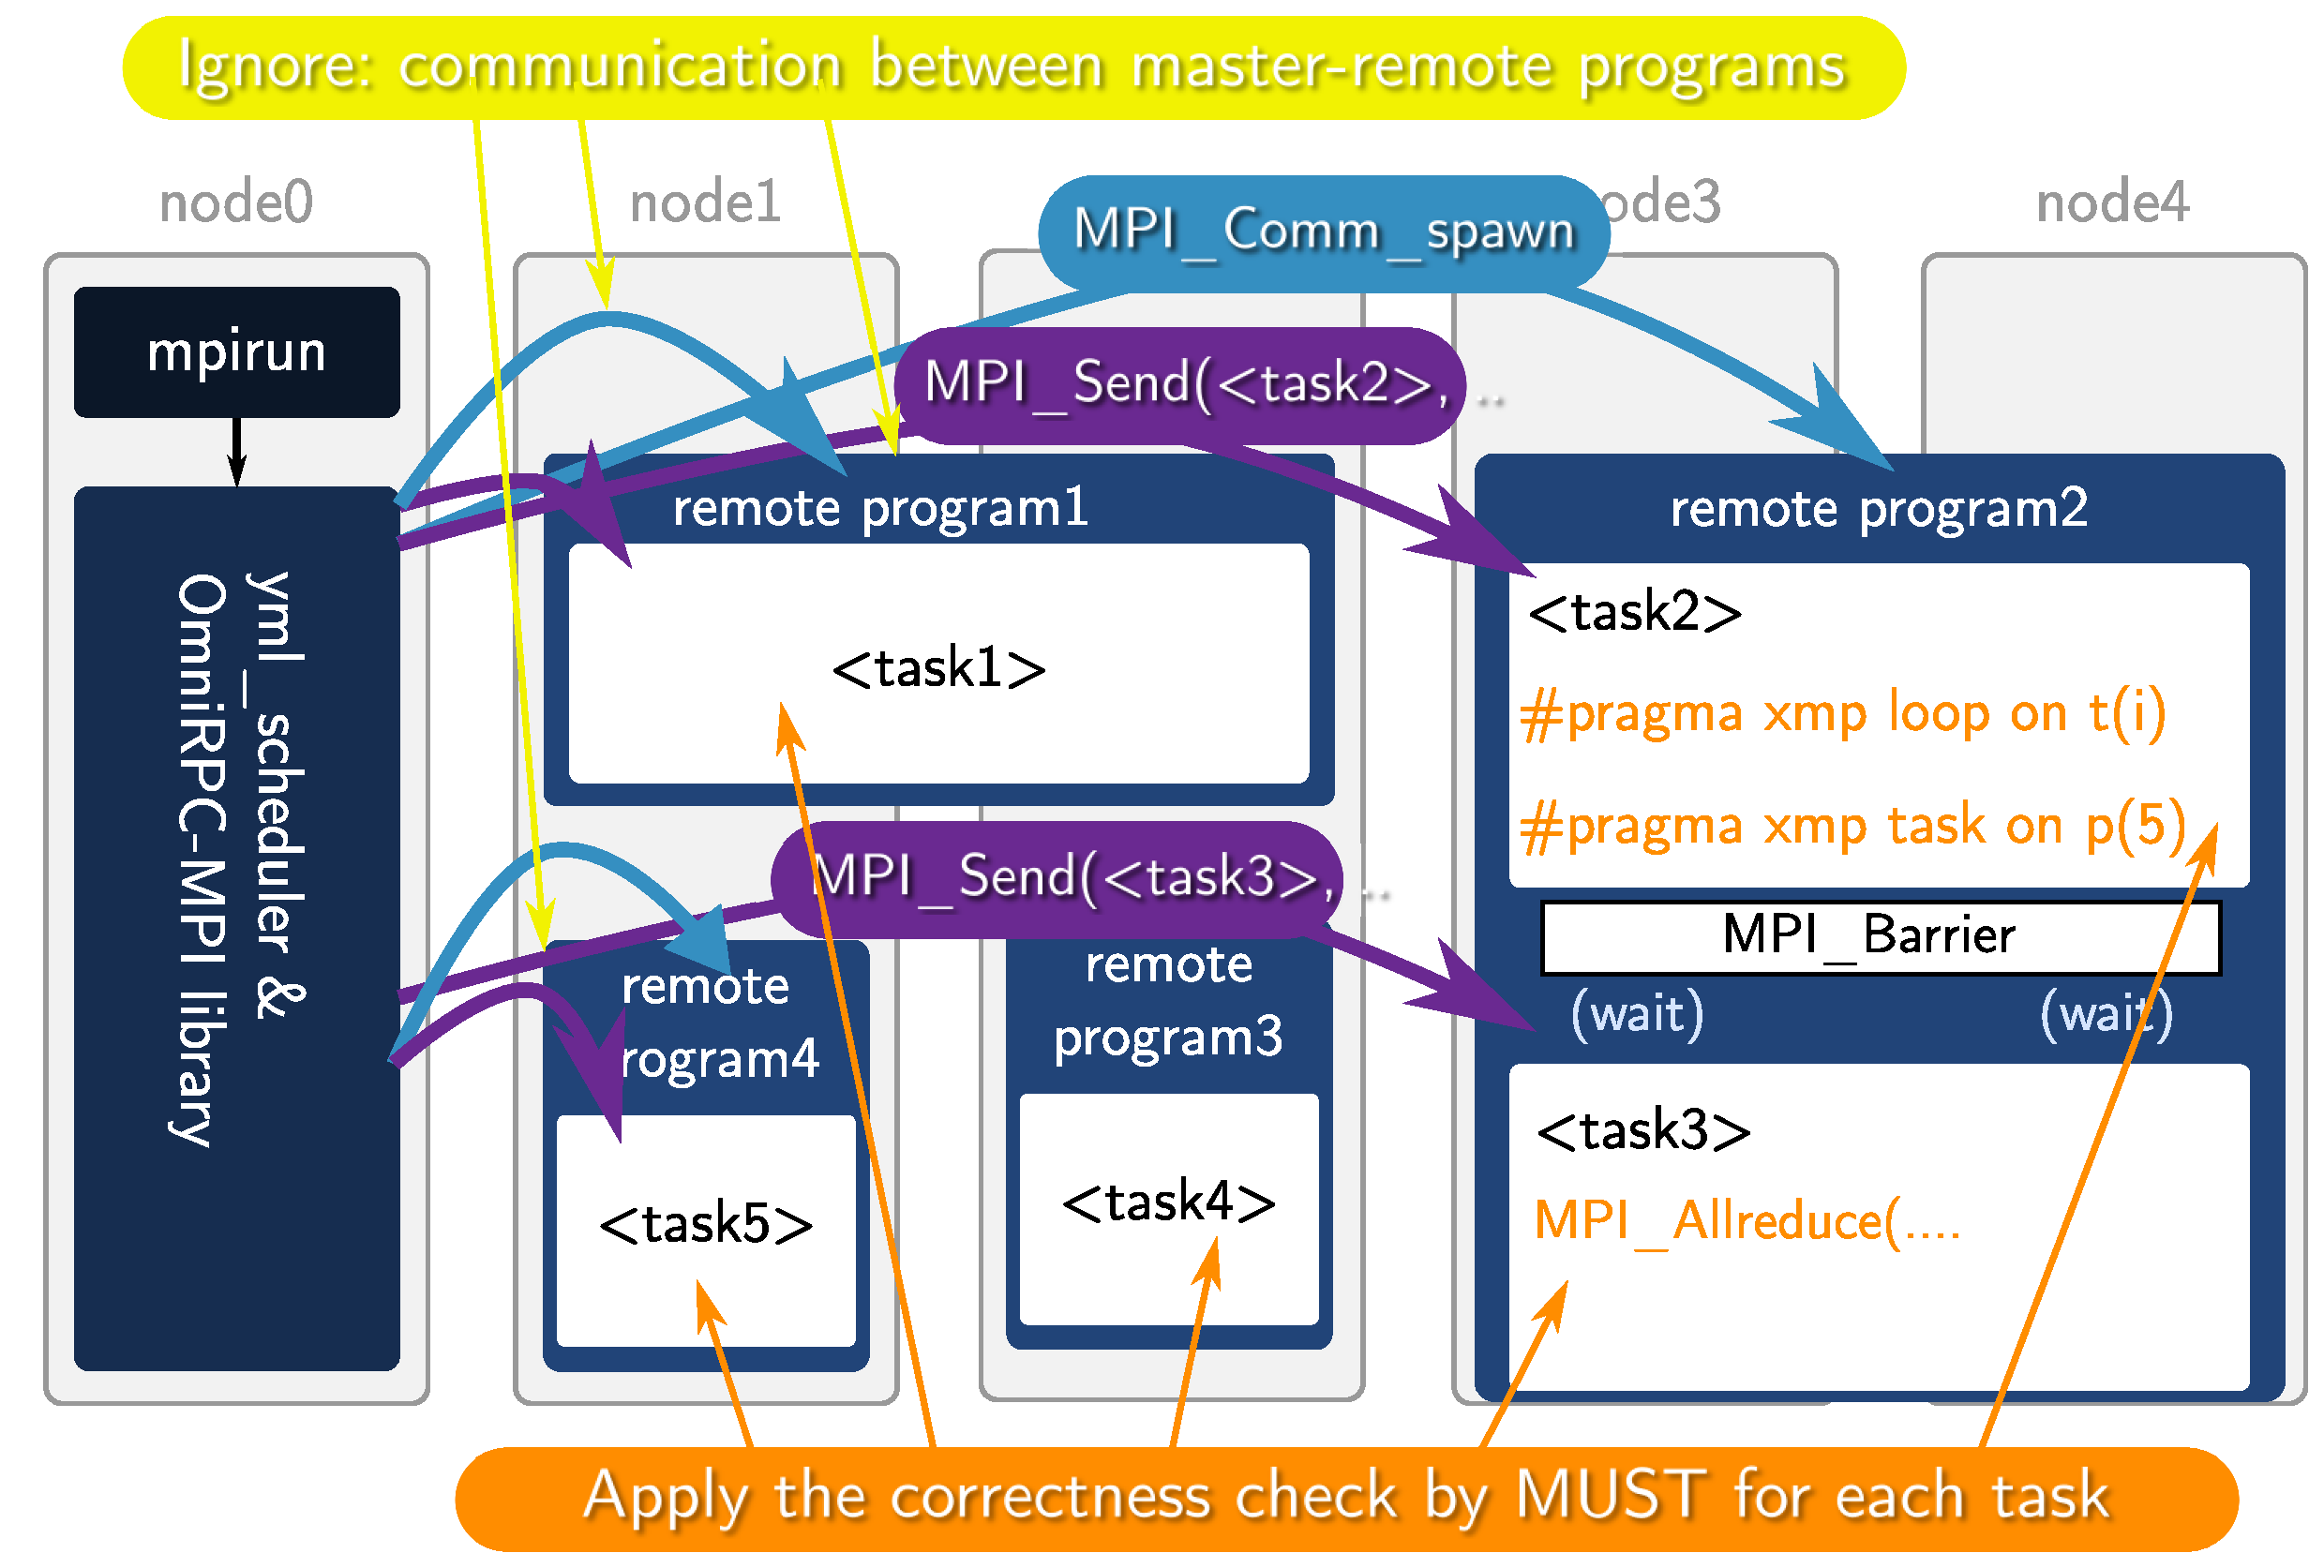
\includegraphics{img/myx-workflow.eps}}
\caption{
Range in application of the correctness checking by MUST in the mSPMD programming model. 
Only for communication written in red letters are checked, MPI functions written in black letters are not checked.
}
\label{fig:must-target}
 \end{center}
\end{figure}

The mSPMD programming model consists of workflow scheduler, middleware, remote programs, and so on. 
Each of the remote programs includes user-defined tasks and control sections where the remote program communicates with the workflow scheduler. 
In this work, we focus on the user-defined tasks within the remote programs and the correctness check by the MUST library should be applied only to the user-defined tasks. Fig. \ref{fig:must-target} shows an overview of the application execution in the mSPMD programming model and the target of the correctness check by the MUST library in the mSPMD programming model. While the MPI and XMP communications shown in orange letters are checked by MUST, MPI\_Comm\_spawn used to invoke remote programs, MPI\_Send used to send a request to the remote programs, must be ignored. 

\begin{figure}[t]
\begin{center}
\scalebox{0.2}{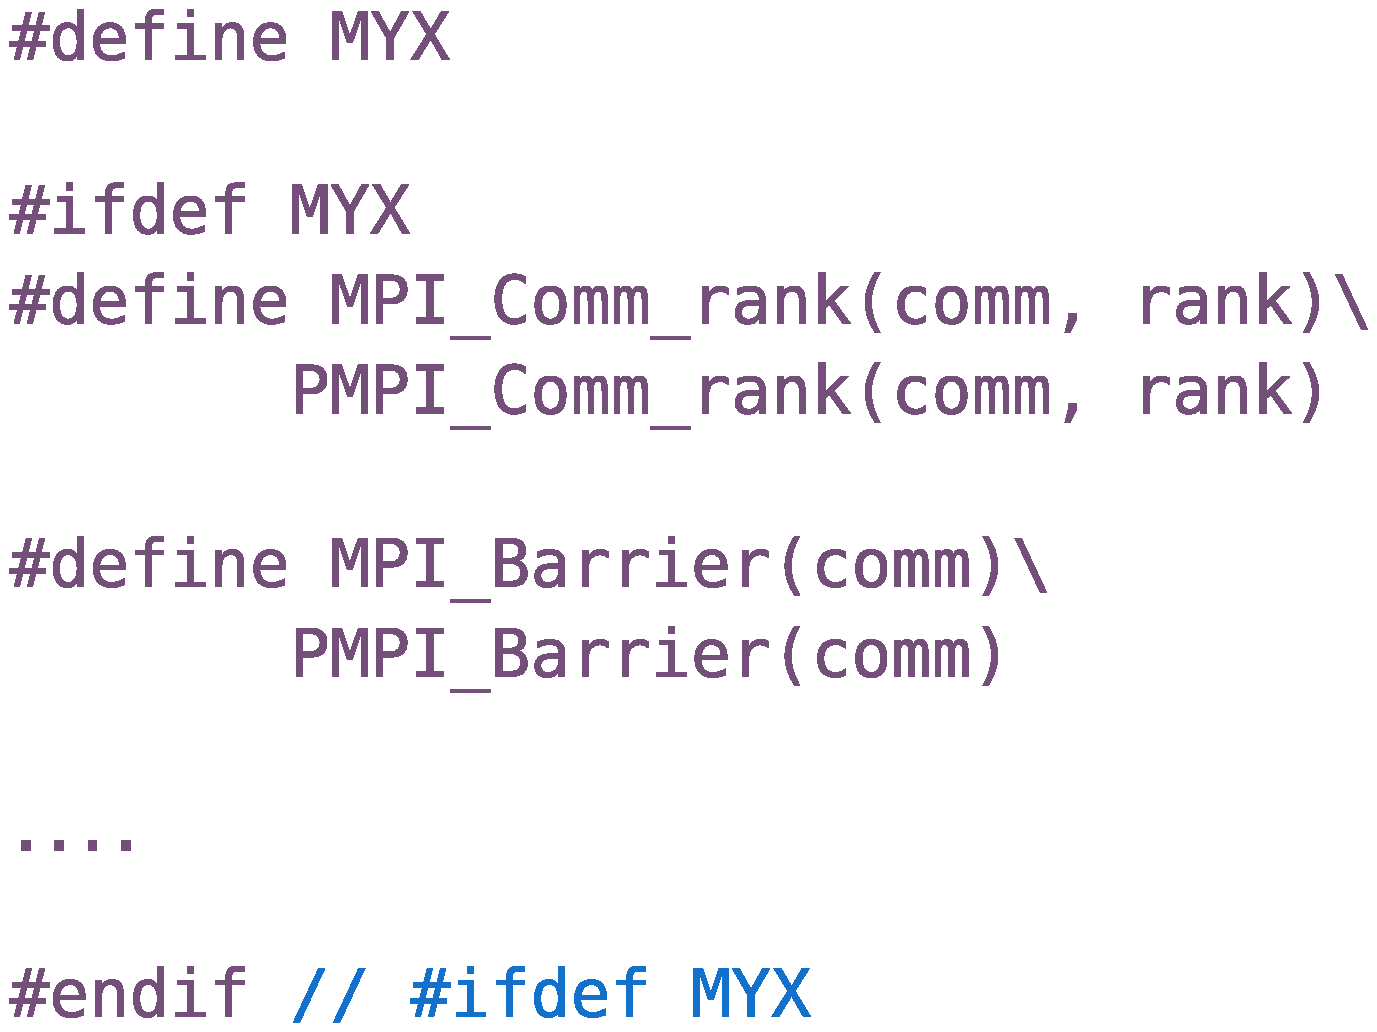
\includegraphics[bb=0 0 661 495]{img/myx-wrapper1.pdf}}
\caption{The Macro to disable the MUST correctness check}
\label{fig:must-wrapper1}
~\\
\scalebox{0.22}{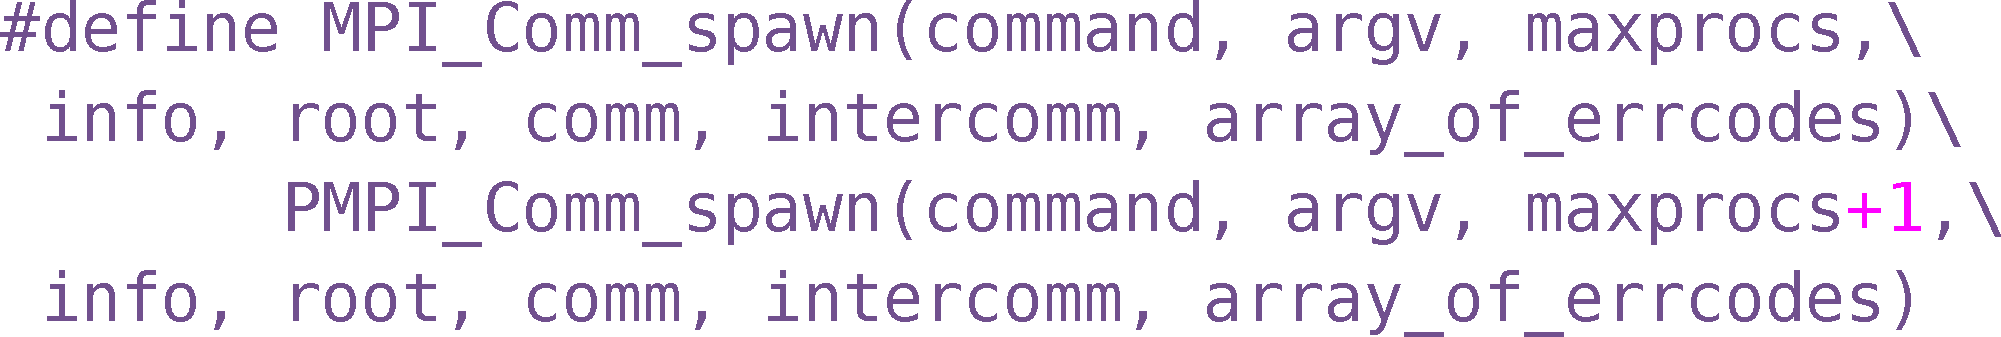
\includegraphics[bb=0 0 961 162]{img/myx-wrapper2.pdf}}
\caption{The Macro to invoke remote programs with $n+1$ processes where ``+1'' is kept for MUST}
\label{fig:must-wrapper2}
\end{center}
\end{figure}

MUST replaces MPI functions starting with MPI\_ such as MPI\_Send with their own MPI functions include correctness check and real communication. 
The functions starting with MPI\_ such as MPI\_Send in standard MPI libraries wrap the functions starting with PMPI\_ which perform communication. 
In order to avoid the correctness check for the control sections, we define some macro to use PMPI functions directly (Figure \ref{fig:must-wrapper1}). Moreover, to reserve an additional process for MUST in remote programs, we define the macro to invoke remote programs (\ref{fig:must-wrapper2}). 

\begin{figure}[t]
\begin{center}
\scalebox{0.32}{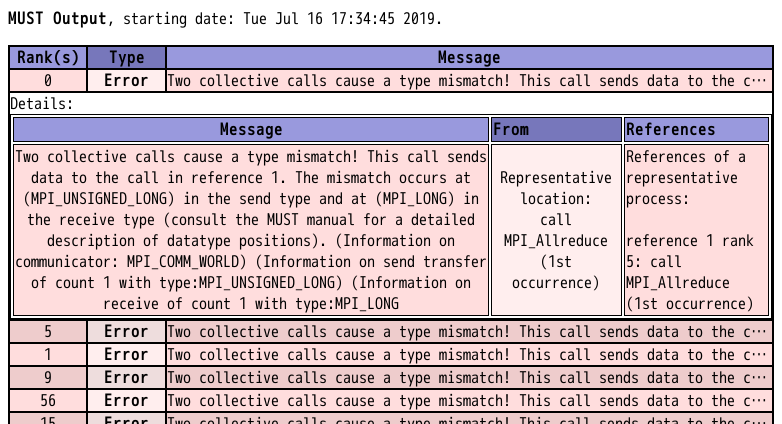
\includegraphics[bb=0 0 782 424]{img/screenshot-allreduce.png}}
\caption{Screenshot of the output file generated by MUST in the mSPMD programming model}
\label{figure:myx-result-screenshot}
\end{center}
\end{figure}

The original MUST gives an output file named {\tt MUST\_Output.html} for each of parallel applications. 
On the other hand, in the mSPMD programming model, there are one or more parallel applications simultaneously. Therefore, we modify the MUST library to generate different {\tt MUST\_Output\_<id>.html} files for different remote programs. So far, we give a process id of the rank-0 of a remote program as the {\tt <id>} the output file. Figure \ref{figure:myx-result-screenshot} shows an example of the output file generated by MUST in the mSPMD programming model. 

\subsection{Experiments}

\begin{table}[t]
\begin{center}
 \caption{The specification of the Oakforest PACS}
 \label{tb:ofp}
\begin{tabular}[t]{rl}\hline\hline
CPU & Intel Xeon Phi 7250 (KNL), 68 core, 1.4 GHz\\
Memory & 96GB(DDR) + 16GB(MCDRAM)\\
Network  & Intel Omni-Path Network, 100 Gpbs\\
Compiler & intel/2018.1.163\\
MPI library & impi/2018.1.163\\
OS & CentOS 7\\\hline
\end{tabular}
\end{center}
\end{table}

We have performed some experiments to evaluate the execution times and to investigate applications' behaviors with and without the MUST library. 
In these experiments, the Oakforest-PACS (OFP) system has been used. Table \ref{tb:ofp} shows the specification of the OFP. For remote programs, we adopt the flat-MPI programming model where each MPI process runs on each core. 
 
\begin{figure}[t]
 \begin{center}
  \scalebox{0.3}{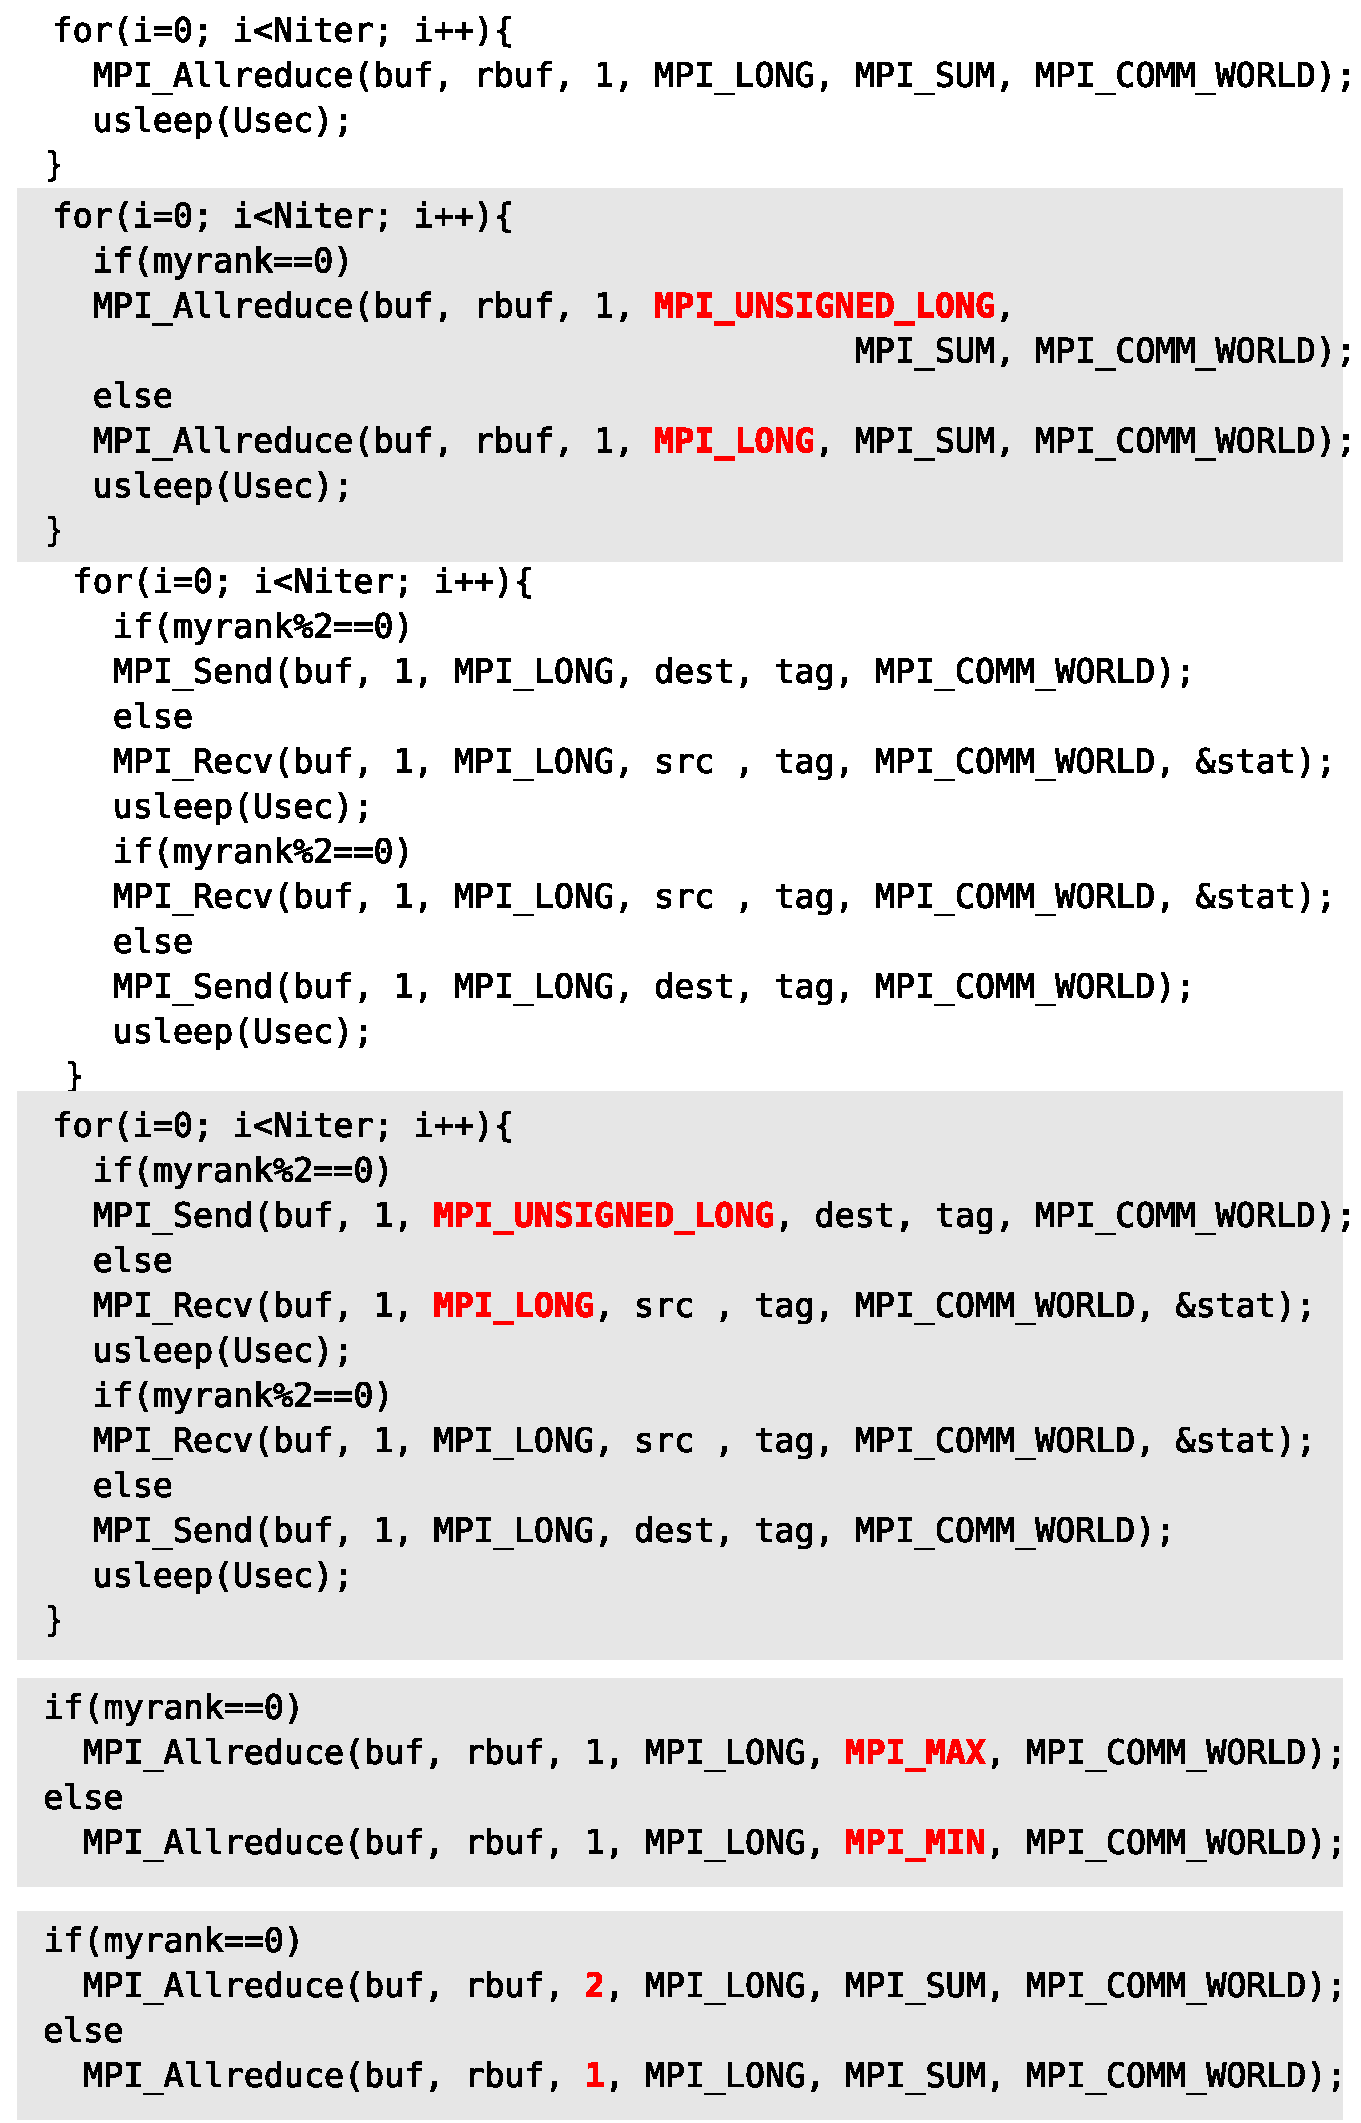
\includegraphics[bb=0 0 653 1019]{img/code-test.pdf}}
\caption{The tasks used in experiments. From the top to bottom, allreduce (w/o error), allreduce (w/ data type error), pingpong (w/o error), and pingpong (w/ error), allreduce (w/ operation error), allreduce (w/ data size error)}
  \label{fig:test-tasks}
 \end{center}
\end{figure}

We focus on collective communication (MPI\_Allreduce) and point-to-point communication (Pingpong), and consider codes with and without error for each. 
Fig. \ref{fig:test-tasks} shows the tasks used in the experiments. 
From the top to bottom, allreduce (w/o error), allreduce (w/ error, type mismatch), pingpong (w/o error), pingpong (w/ error, type mismatch), allreduce (w/ error, operation mismatch), and allreduce (w/ error, buffer size mismatch). 
Also, we consider different numbers of iterations, and different interval seconds between MPI function calls in each test codes for the overhead evaluations. 

\begin{table}[t]
\caption{Applications' behaviors and the statuses of error reports}
\label{table:stats}
 \begin{center}
  \begin{tabular}[t]{|r|r|r|}\hline\hline
   & w/ MUST & w/o MUST \\\hline
  allreduce w/o error & completed & completed \\\hline
  allreduce w/~ & completed & completed \\
  type conflict error &  error reports & no report\\\hline
  pingpong w/o error & completed & completed \\\hline
  pingpong w/~ & completed & completed \\
  type conflict error &  error reports &  no report\\\hline
  allreduce w/~ & completed & completed \\
  operation conflict error &  error reports &  no report\\\hline
  allreduce w/~ & failed & failed \\
  buffer size conflict error & error reports  & simple error reports \\\hline
  \end{tabular}
 \end{center}
\end{table}

Table \ref{table:stats} shows the applications' behaviors and the statuses of error reports, when applying or not applying MUST.
While the datatype conflict and operation conflict errors are reported when we apply the MUST, the applications are completed without any report when we don't apply the MUST even though the results of the reduction should be wrong. 

\begin{figure}[t]
 \begin{center}
\scalebox{1.0}{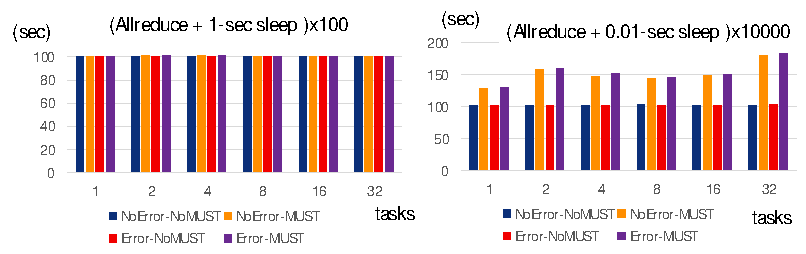
\includegraphics{img/myx-allreduce.eps}}  
\caption{Execution time when a workflow includes $1, 2, \cdots 32$ tasks executing MPI\_Allreduce repeatedly every 1-sec (left) and every 0.01-sec }
\label{fig:result-myx allreduce}
~\\
\scalebox{1.0}{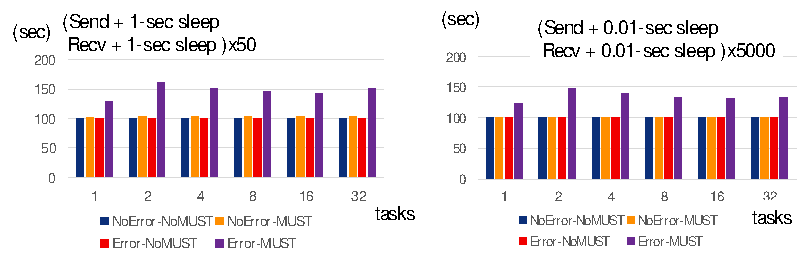
\includegraphics{img/myx-sendrecv.eps}}  
\caption{Execution time when a workflow includes $1, 2, \cdots 32$ tasks executing MPI\_Send/Recv repeatedly every 1-sec (left) and every 0.01-sec }
\label{fig:result-myx pingpong}
 \end{center}
\end{figure}

Figure \ref{fig:result-myx allreduce} shows the execution time of the mSPMD programming executions with and without the MUST library. Workflow applications include between 1 and 32 tasks of MPI\_Allreduce. 
Figure \ref{fig:result-myx pingpong} shows the results for MPI\_Send/Recv. 
Each task uses 32 processes in the all experiments. 
As shown in the figure \ref{fig:result-myx allreduce}, the overhead to check and record errors of the collective communication is ignorable if we don't perform communication very intensively. On the other hand, if collective communication functions called very freqently, then the overheads become large even if there is no error. 
As shown in the figure \ref{fig:result-myx pingpong}, the overhead of the MUST libary is small if there is no error in point to point communication functions.  However, it takes longer time if there is some errors. The fact indicate that there is almost no overhead to check point to point communication, but it takes some time to analyze and record errors in the point to point communicaiton functions. 

\section{Summary}

In this chapter, we have introduced the mSPMD programming model and programming environment, where several SPMD programs work together under control of a workflow program. YML, which is a development and execution environment for scientific workflows, and its middleware OmniRPC, have been extended to manage several SPMD tasks and programs. 
As well as MPI, XMP, a directive based parallel programming language, has been supported to describe tasks. 
A task generator has been developed to incorporate XMP programs into a workflow. 
Fault tolerant features, correctness check, and some numerical libraries' implementations in the mSPMD programming model have been presented. 


%\bibliographystyle{plain} 
%\bibliography{bib}

\begin{thebibliography}{10}

\bibitem{Augonnet2011starpu}
C{\'e}dric Augonnet, Samuel Thibault, Raymond Namyst, and Pierre-Andr{\'e}
  Wacrenier.
\newblock {StarPU: A Unified Platform for Task Scheduling on Heterogeneous
  Multicore Architectures}.
\newblock {\em Concurrency and Computation: Practice and Experience - Euro-Par
  2009}, 23:187--198, 2011.

\bibitem{delannoy2006b}
Olivier Delannoy.
\newblock {\em YML: A scientific Workflow for High Performance Computing}.
\newblock PhD thesis, University of Versailles Saint-Quentin, 2006.

\bibitem{delannoy2006a}
Olivier Delannoy, Nahid Emad, and Serge Petiton.
\newblock Workflow global computing with yml.
\newblock In {\em The 7th IEEE/ACM International Conference on Grid Computing},
  pages 25--32, 2006.

\bibitem{delannoy2004a}
Olivier Delannoy and Serge Petiton.
\newblock A peer to peer computing framework: Design and performance evaluation
  of yml.
\newblock In {\em 3rd International Workshop on Algorithms, Models and Tools
  for Parallel Computing on Heterogeneous Networks}, pages 362--369, 2004.

\bibitem{Hilbrich2013must}
Tobias Hilbrich, Fabian Hasel, Martin Schulz, Bronis~R. de~Supinski,
  Matthias~S. Muller, and Wolfgang~E. Nagel.
\newblock Runtime {MPI} collective checking with tree-based overlay networks.
\newblock In {\em Proceedings of the 20th European MPI Users' Group Meeting
  (EuroMPI 13)}, pages 129--134. ACM, 2013.

\bibitem{Hilbrich2012must}
Tobias Hilbrich, Joachim Protze, Martin Schulz, Bronis~R. de~Supinski, and
  Matthias~S. Muller.
\newblock {MPI} runtime error detection with {MUST}: Advances in deadlock
  detection.
\newblock In {\em International Conference on High Performance Computing,
  Networking, Storage and Analysis (SC12)}. IEEE, 2012.

\bibitem{odajima2013Adaptive}
Tetsuya Odajima, Taisuke Boku, Mitsuhisa Sato, Toshihiro Hanawa, Yuetsu Kodama,
  Raymond Namyst, Samuel Thibault, and Olivier Aumage.
\newblock Adaptive task size control on high level programming for gpu/cpu work
  sharing.
\newblock In {\em International Symposium on Advances of Distributed and
  Parallel Computing (ADPC 2013)}, pages 59--68, 2013.

\bibitem{Protze2017a}
Joachim Protze, Christian Terboven, Matthias~S. M{\"u}ller, Serge Petiton,
  Nahid Emad, Hitoshi Murai, and Taisuke Boku.
\newblock Runtime correctness checking for emerging programming paradigms.
\newblock In {\em Proceedings of the First International Workshop on Software
  Correctness for HPC Applications}, pages 21--27, 2017.

\bibitem{sato2001a}
Mitsuhisa Sato, Motonari Hirano, Yoshio Tanaka, and Satoshi Sekiguchi.
\newblock Omnirpc: A grid rpc facility for cluster and global computing in
  openmp.
\newblock In {\em International Workshop on OpenMP Applications and Tools,
  2001}, pages 130--136, 2001.

\bibitem{Sorensen-iram}
Danny~C. Sorensen.
\newblock {\em ICASE/LaRC Interdisciplinary Series in Science and Engineering
  book series (ICAS, volume 4)}, chapter Implicitly Restarted Arnoldi/Lanczos
  Methods for Large Scale Eigenvalue Calculations, pages 119--165.
\newblock springer, 1997.

\bibitem{matrix-collection}
{SuiteSparse Matrix Collection}.
\newblock {https://sparse.tamu.edu/}.

\bibitem{MUST-project}
{The MUST Project}.
\newblock https://www.itc.rwth-aachen.de/must.

\bibitem{tsuji2015i}
Miwako Tsuji, Serge Petiton, and Mitsuhisa Sato.
\newblock Fault tolerance features of a new multi-spmd programming/execution
  environment.
\newblock In {\em Proceedings of the First International Workshop on Extreme
  Scale Programming Models and Middleware SC15}, pages pp.20--27
  doi:10.1145/2832241.2832243. ACM, 2015.

\bibitem{tsuji2013c}
Miwako Tsuji, Mitsuhisa Sato, Maxime Hugues, and Serge Petiton.
\newblock Multiple-spmd programming environment based on p{GA}s and workflow
  toward post-petascale computing.
\newblock In {\em Proceedings of the 2013 International Conference on Parallel
  Processing (ICPP-2013)}, pages 480--485. IEEE, 2013.

\end{thebibliography}


\end{document}